\documentclass[fleqn,10pt]{wlscirep}
\usepackage[utf8]{inputenc}
\usepackage[T1]{fontenc}
\usepackage{multirow}
\usepackage{graphicx}
\usepackage{subcaption}
\usepackage{float}
\hfuzz=1pt
\hbadness=10000
\title{APEXPSO: Adaptive Parameter Exploration with CrossQ-SAC for UAV Path Planning via Particle Swarm Optimization}

\author[1,*]{Alice Author}
\author[2]{Bob Author}
\author[1,2,+]{Christine Author}
\author[2,+]{Derek Author}
\affil[1]{Affiliation, department, city, postcode, country}
\affil[2]{Affiliation, department, city, postcode, country}

\affil[*]{corresponding.author@email.example}

\affil[+]{these authors contributed equally to this work}

%\keywords{Particle Swarm Optimization, Deep Reinforcement Learning, Soft Actor-Critic, UAV Path Planning, Parameter Adaptation}

\begin{abstract}
Particle Swarm Optimization (PSO) is widely used for UAV path planning, but its performance critically depends on control parameters that traditionally require manual tuning or follow fixed schedules.
While recent reinforcement learning approaches have shown promise in adaptive parameter control, they have not fully exploited state-of-the-art deep RL advances.
We present APEXPSO (Advanced Parameter Exploration with CrossQ-SAC for PSO), a novel framework that combines Soft Actor-Critic with CrossQ optimizations, transformer-based state encoding, and multi-objective reward design for per-particle parameter adaptation in UAV path planning.
Our approach uses a 45-dimensional state representation with multi-head attention over temporal windows to capture swarm dynamics, outputting per-particle control parameters in a 120-dimensional continuous action space.
Comprehensive ablation studies demonstrate that while the multi-objective reward is critical, a simpler state representation often rivals the attention mechanism, and simpler parameter granularity (5-subgroup control) surprisingly outperforms fine-grained per-particle adaptation.
APEXPSO achieves superior path quality with reduced manual tuning compared to traditional PSO variants and learning-based baselines, advancing the state-of-the-art in adaptive metaheuristic control for autonomous navigation.
\end{abstract}
\begin{document}
\raggedbottom

\flushbottom
\maketitle
% * <john.hammersley@gmail.com> 2015-02-09T12:07:31.197Z:
%
%  Click the title above to edit the author information and abstract
%
\thispagestyle{empty}

\section*{Introduction}
\label{sec:intro}
  
Unmanned Aerial Vehicles (UAVs) support missions ranging from precision agriculture to defense and disaster response \cite{Delavarpour2021, Fascista2022, Alotaibi2019}.
Every mission hinges on path planning to compute safe, constraint-aware trajectories through cluttered three-dimensional environments.
Despite decades of study, planning in large, uncertain airspaces remains difficult because algorithms must simultaneously reason about vehicle dynamics, environmental constraints, and mission-specific trade-offs. 
A rich ecosystem of planners has emerged to tackle these demands, spanning heuristic graphs, sampling-based motion planners, bio-inspired swarms, and learning-enabled controllers \cite{AitSaadi2022}.

Prior surveys catalog the breadth of UAV motion planning strategies, emphasizing how dynamic feasibility, mapping representations, and trajectory optimization challenges shape practical mission performance \cite{Zhou2025UAVMotionPlanning}.
These studies emphasize that planners must reason about aerodynamic and kinematic constraints \cite{Zhou2025UAVMotionPlanning} while exploiting terrain awareness and sensor feedback to guarantee safe arrivals \cite{pathplanning_review2}.
Classical graph-search heuristics such as A* and its informed variants remain attractive for grid-based maps because they provide completeness and, in some cases, optimality guarantees \cite{pathplanning_review1,pathplanning_review2,Hart1968}.
Sampling-based planners such as RRT and PRM are better suited to high-dimensional workspaces, as are stochastic motion planners that sample candidate waypoints or trajectories \cite{Faust2017}.
These techniques trade determinism for coverage, enabling planners to respond to large, partially known environments.
Bio-inspired and learning-driven approaches push further by embedding adaptation into the search itself.
Evolutionary schemes (Differential Evolution, Genetic Algorithms) evolve path encodings to satisfy safety and energy constraints \cite{Debnath2024GAUAV}, while swarm-intelligence algorithms (PSO, ACO, GWO) coordinate collectives of candidate solutions dynamic-inertia tuning \cite{Bansal2011}, illustrate how domain-specific knowledge can be fused with stochastic search to handle tight turning, altitude, or threat envelopes.

Particle Swarm Optimization (PSO) \cite{kennedy1995pso} exemplifies such hybrid potential.
PSO is widely cited for its fast convergence and adaptability in complex UAV path planning problems \cite{Cheng2024UAVPSO}.
However, PSO's performance relies on carefully tuned inertia and acceleration coefficients, which are notoriously problem-dependent and can cause premature convergence when left static \cite{yang2015lhnpso}.
Adaptive parameter control is therefore essential to unlock PSO's robustness.
In this research, we introduce an advanced parameter exploration with CrossQ-SAC for PSO (APEX-PSO), a deep reinforcement learning framework that learns PSO control policies directly from swarm feedback.
Our contributions are fourfold: (i) a CrossQ-enhanced Soft Actor-Critic agent that improves sample efficiency via batch-normalized critics, (ii) a transformer-based state encoder that captures temporal swarm dynamics, (iii) a multi-objective reward that balances fitness gains, diversity, convergence speed, and curiosity, and (iv) a study of parameter-granularity settings ranging from global to per-particle control.
Extensive experiments on 3D terrain navigation benchmarks show that APEXPSO delivers higher-quality paths with far less manual tuning than heuristic schedules or prior RL controllers.
The subsequent results highlight that while the multi-objective reward is critical, the complex attention mechanism does not consistently outperform a simpler state representation, suggesting that immediate swarm statistics are often sufficient for effective control. Furthermore, the 5-subgroup granularity mode consistently outperforms or matches the per-particle variant while requiring fewer action dimensions (Table \ref{tab:rl_comparison}), confirming the practical trade-offs we target for *Swarm and Evolutionary Computation* readers.

The remainder of this paper reviews related work in \hyperref[sec:background]{Background and Related Work}, presents the APEXPSO methodology in \hyperref[sec:methods]{Methods}, reports experimental findings in \hyperref[sec:results]{Results}, and concludes with discussion and future directions in \hyperref[sec:discussion]{Discussion}.
\section*{Background and Related Work}
\label{sec:background}

\subsection*{Particle Swarm Optimization}

Particle Swarm Optimization (PSO) is a population-based stochastic search inspired by social behaviors of flocks and swarms \cite{kennedy1995pso}.
In PSO, a swarm of candidate solutions (particles) moves through the search space by updating its velocity and position based on each particle's own best-found solution (cognitive component) and the swarm's best-found solution (social component).
An inertia term maintains momentum between successive updates \cite{clerc2002stagnation}.
The velocity and position updates follow:
\begin{equation}
\left\{
\begin{aligned}
v_i^{t+1} &= w\,v_i^{t} + c_1 r_1^{t}\odot(p_i^{t}-x_i^{t}) + c_2 r_2^{t}\odot(g^{t}-x_i^{t}),\\
x_i^{t+1}&=x_i^{t}+v_i^{t+1}.
\end{aligned}
\right.
\end{equation}
Here, \(w\) is the inertia weight, \(c_1\) and \(c_2\) are the cognitive and social coefficients, and \(r_1,r_2\) are random vectors.
Because PSO performance critically depends on its control parameters, a rich body of work focuses on how to set or adapt \(w\), \(c_1\), and \(c_2\) during the search.
Parameter setting methods fall into two broad categories: parameter tuning and parameter control \cite{Eberhart2000parametercontrol}.
Unlike static tuning, parameter control methods monitor the swarm's behavior and adjust parameters to balance exploration and exploitation in response to the search state \cite{Nickabadi2011a}. 
A robust parameter schedule must preserve diversity early on (high \(w\), modest \(c_1\)) while allowing rapid convergence later (lower \(w\), higher \(c_2\)).
However, manually designed schedules struggle to generalize across terrains and obstacle densities, and they cannot react if individual particles stagnate or diverge.
Learning-based adaptation treats each PSO iteration as a decision point: the controller observes summary statistics of the swarm, predicts suitable \(w,c_1,c_2\) values (with optional granularity from global to per-particle), and immediately applies them before the next velocity update.
This perspective motivates the architecture in Section \ref{sec:methods}, where we encode temporal swarm states with a transformer and deploy a CrossQ-enhanced Soft Actor-Critic agent to learn the policy; Section \ref{sec:results} then evaluates different granularity modes to show how subgroup-level control often outperforms a heavy per-particle policy while staying tractable.

A classical approach is to use a time-varying schedule.
For example, a linearly decreasing inertia weight \(w\) encourages global exploration initially (high \(w\)) and emphasizes exploitation later (low \(w\)) \cite{Eberhart2000parametercontrol}.
Similarly, time-varying acceleration coefficients (TVAC) have been introduced to gradually increase the social weight \(c_2\) and decrease the cognitive weight \(c_1\) over time \cite{ratnaweera2004tvac}.
These schemes are easy to implement and capture the intuition that early search should be explorative and later search more greedy.
Sinusoidal and periodic time-varying parameter schedules have been explored extensively in PSO, ranging from oscillating inertia weights \cite{kentzoglanakis2009oscillating} to sinusoidally varying acceleration coefficients \cite{chen2018sinusoidal}, and offer a principled way to introduce smooth cyclic transitions between exploratory and exploitative behavior.
Recent PSO extensions, including spherical-vector control \cite{manh2022sphericalpso} and dynamic-inertia tuning \cite{Bansal2011}, illustrate how domain-specific knowledge can be fused with stochastic search to handle tight turning, altitude, or threat envelopes.
Beyond hand-designed schedules, adaptive and self-adaptive PSO strategies use feedback from the swarm to dynamically adjust parameters during optimization.
Fitness-based adaptation adjusts parameters such as inertia weight or acceleration coefficients according to the relative performance of particles, allowing better-performing individuals to guide the swarm more strongly while underperforming particles explore alternative regions \cite{Li2017particle}.
Recent literature successfully combines these methods.
Liu et al. \cite{Liu2025spherical} proposed per-particle parameter adaptation based on fitness adaptation parameter $fap_i^{t}$ that normalizes individual's fitness relative to the global best and average fitness with sinusoidal bounds $\chi^{t}$ which is an adaptive sine factor that creates smooth sinusoidal time-varying modulation:
\begin{equation}
\left\{
\begin{aligned}
    \omega_i^{t}&=\omega_{max}-(\omega_{max}-\omega_{min})\cdot\frac{t}{T}\cdot fap_i^{t},\\
    c_{1,i}^{t}&=c_{max}-(c_{max}-c_{min})\cdot \chi^{t} \cdot fap_i^{t},\\
    c_{2,i}^{t}&=c_{min}+(c_{max}-c_{min})\cdot \chi^{t} \cdot fap_i^{t}.
\end{aligned}
\right.
\end{equation}
This mechanism enables per-particle parameter heterogeneity in two ways.
First, the fitness adaptation parameter $fap_i^{t}$ ensures that better-performing particles receive different $\omega$, $c_1$, and $c_2$ values compared to worse-performing particles.
Second, the sinusoidal factor $\chi^{t}$ creates a smooth temporal progression.
In early iterations, $\chi^{t}$ emphasizes personal learning, while in later iterations it shifts emphasis to social learning, enabling particles to balance exploration and exploitation dynamically across the entire optimization process.
Isiet and Gadala's Unique Adaptive PSO (UAPSO) \cite{Isiet2019UAPSO} pushes this idea further by deriving every particle's control parameters from an evolutionary-state metric.
Each particle stores the fitness of its latest feasible position $f(x^{t}_{i,\mathrm{feas}})$ and computes
\begin{equation}
ES_i^{t} = \frac{f(p_i^{t}) - f(g^{t})}{f(x^{t}_{i,\mathrm{feas}})},
\end{equation}
which simultaneously acts as the particle's inertia weight ($w_i^{t}=ES_i^{t}$) and drives a piecewise time-varying schedule for the acceleration coefficients:
\begin{equation}
\left\{
\begin{aligned}
    c_{1,i}^{t} &=
        \begin{cases}
            (c_{\max}-c_{\min})\frac{T-t}{T} + c_{\min}, & ES_i^{t} \le 0.5,\\
            c_{\max} - (c_{\max}-c_{\min})\frac{T-t}{T}, & ES_i^{t} > 0.5,
        \end{cases} \\[6pt]
    c_{2,i}^{t} &=
        \begin{cases}
            c_{\max} - (c_{\max}-c_{\min})\frac{T-t}{T}, & ES_i^{t} \le 0.5,\\
            (c_{\max}-c_{\min})\frac{T-t}{T} + c_{\min}, & ES_i^{t} > 0.5.
        \end{cases}
\end{aligned}
\right.
\end{equation}
Particles with low $ES_i^{t}$ (far from both their personal best and the global leader) therefore receive small inertia weights and large social pulls, whereas particles with high $ES_i^{t}$ maintain higher momentum and stronger cognitive influence.
A repulsion term $(1-ES_i^{t})(g^{t}-p_i^{t})$ is also applied to discourage swarm clustering.
On structural design and CEC benchmarks, UAPSO consistently achieves lower mean fitness, reduced variance, and more frequent best-solution hits than the time-varying PSO baselines.
Despite these advances, fundamental challenges persist in self-adaptive PSO design.
The convergence behavior of many SAPSO algorithms remains poorly understood, with analytical and empirical studies revealing that adapted parameters often fail to reach stable points or adhere to well-known convergence criteria~\cite{harrison2018sapso}.
The development of truly parameter-free PSO algorithms continues to be hindered by the complexity of predicting long-term parameter performance based on limited short-term information, necessitating ongoing research into more robust adaptive mechanisms that can balance exploration and exploitation without introducing additional tuning burdens.

Beyond standard fitness-based adaptation, recent advancements have introduced control mechanisms driven by more complex swarm metrics.
Entropy-based strategies monitor the disorder of the swarm's distribution to dynamically adjust weights, preventing stagnation by injecting diversity when system entropy drops below critical thresholds \cite{Han2022Entropy}.
Success-rate based control, such as the Adaptive Inertia Weight PSO (AIWPSO), utilizes the historical improvement rate of individual particles as a feedback signal, effectively distinguishing between successful foragers and those trapped in local optima to assign heterogeneous parameter values \cite{Li2019AIWPSO}.
More granular control is achieved through evolutionary state estimation (ESE), notably employed in the APSO-ZZLC algorithm, which classifies the search process into four distinct stages---exploration, exploitation, convergence, and jumping out---using fuzzy membership functions to apply state-specific parameter adaptation rules \cite{Zhan2009APSO}.
To address the uncertainty of selecting a single adaptation strategy, Ensemble PSO (EPSO) frameworks maintain a pool of diverse parameter update strategies, allowing particles to adaptively select the most effective strategy based on online performance rewards \cite{Lynn2017EPSO}.
Crucially, the stability of these adaptive mechanisms is often evaluated against theoretical convergence criteria, such as the stability analysis by Clerc and Kennedy, which defines the precise mathematical relationship between $\omega$, $c_1$, and $c_2$ required to guarantee equilibrium in the particle dynamics \cite{clerc2002stagnation}.

\begin{figure}[H]
\centering
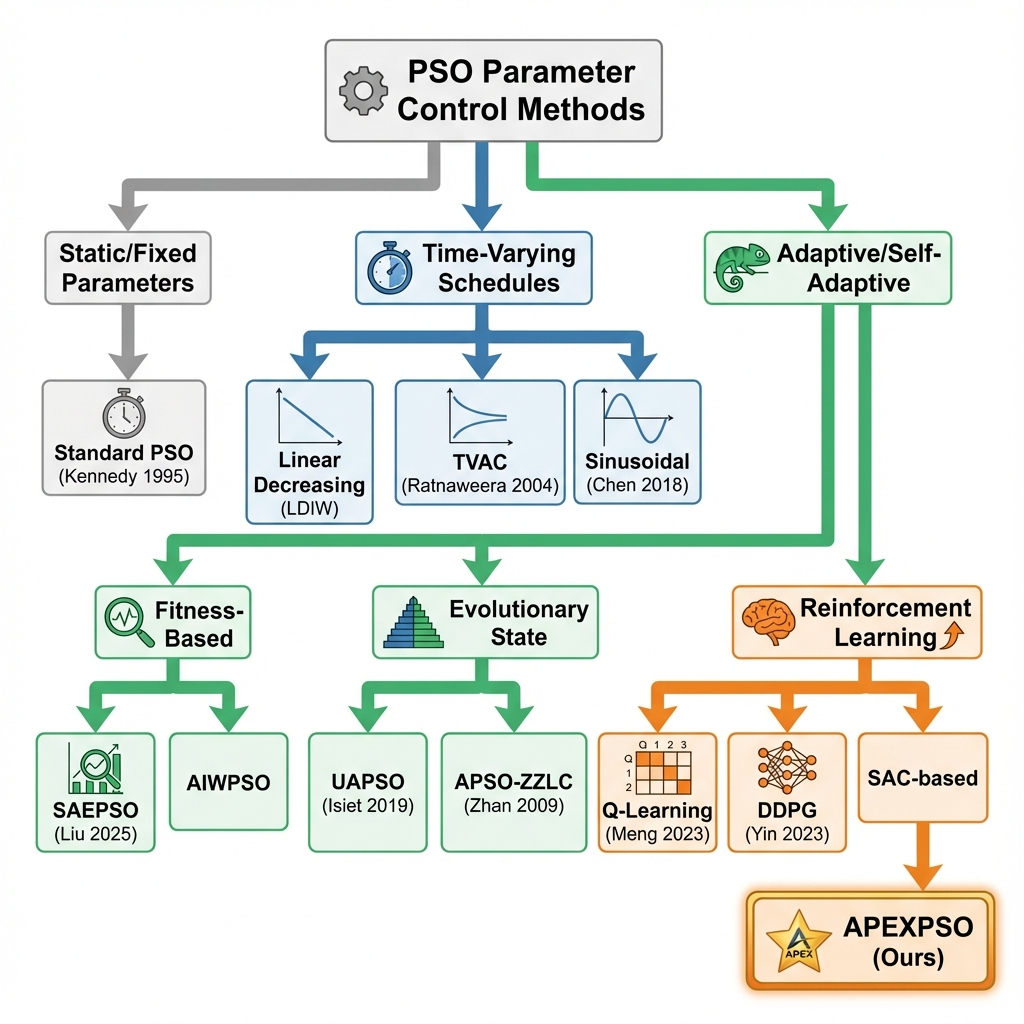
\includegraphics[width=0.95\textwidth]{figures/generated_figure/pso_taxonomy.png}
\caption{Taxonomy of PSO parameter control methods. Static approaches use fixed parameters throughout optimization. Time-varying schedules adjust parameters based on iteration count. Adaptive methods use swarm feedback (fitness-based, evolutionary state) or learned policies (reinforcement learning). APEXPSO (highlighted) combines SAC with CrossQ optimizations and transformer-based state encoding to advance RL-based adaptive control.}
\label{fig:pso_taxonomy}
\end{figure}

Figure~\ref{fig:pso_taxonomy} summarizes the taxonomy of PSO parameter control strategies discussed in this section, highlighting the position of our APEXPSO framework within the reinforcement learning branch.

\subsection*{Reinforcement Learning}

Reinforcement Learning (RL) is a machine learning paradigm where an agent learns to make sequential decisions by interacting with an environment to maximize cumulative rewards \cite{sutton2018rl}.
RL methods have been successfully applied to many fields, including robotics, intelligent algorithms, and control systems.
At each time step $t$, the agent observes a state $s_t$, selects an action $a_t$ according to its policy $\pi(a|s)$, receives a reward $r_{t+1}$, and transitions to a new state $s_{t+1}$.
The goal is to learn an optimal policy $\pi^*$ that maximizes the expected cumulative discounted return $G_t = \sum_{k=0}^{\infty} \gamma^k r_{t+k+1}$.
Value-based methods estimate the action-value function $Q(s,a)$, representing the expected return from taking action $a$ in state $s$.
The classic Q-learning algorithm \cite{watkins1992qlearning} updates Q-values using the Bellman equation:
\begin{equation}
Q(s_t, a_t) \leftarrow Q(s_t, a_t) + \alpha \left[r_{t+1} + \gamma \max_{a'} Q(s_{t+1}, a') - Q(s_t, a_t)\right]
\label{eq:qlearning_update}
\end{equation}
where $\alpha$ is the learning rate and $\gamma \in [0,1]$ is the discount factor.

For continuous action spaces, policy gradient methods directly parameterize the policy $\pi_\theta(a|s)$ and optimize via gradient ascent on the expected return.
Actor-critic architectures combine policy gradients with value function approximation: the actor network learns the policy while the critic network estimates the value function to reduce gradient variance.
Deep Deterministic Policy Gradient (DDPG) \cite{lillicrap2016ddpg} extends this to continuous control with deterministic policies $\mu_\theta(s)$ and experience replay.
Twin Delayed DDPG (TD3) \cite{fujimoto2018td3} addresses overestimation bias through twin critics and delayed policy updates.
Soft Actor-Critic (SAC) \cite{haarnoja2018sac} introduces maximum entropy RL, which augments the objective with policy entropy to encourage exploration, where a temperature parameter $\alpha$ controls the exploration-exploitation balance.

RL has emerged as a powerful paradigm for adaptive parameter control in evolutionary computation, treating the optimizer's configuration as a sequential decision-making problem \cite{Bai2023}.
In this framework, the PSO optimization process serves as the environment: the state encodes swarm statistics, actions correspond to parameter adjustments, and rewards reflect optimization progress.
Early RL-PSO approaches utilized tabular Q-learning with discretized parameter spaces.
Meng et al. \cite{meng2023multi} proposed MPSORL, a multi-strategy self-learning PSO where fitness values define particle states that are non-uniformly divided into subsets, and a Q-table guides strategy selection via $\varepsilon$-greedy action with reward-based updates.
Deep Q-Network (DQN) variants have also been explored: Wu et al. \cite{wu2024dqnpso} introduced DPQ-PSO, which combines DQN with Hidden Markov Models to dynamically tune inertia weight and acceleration coefficients, preventing premature convergence on complex benchmark functions.
However, such discretized methods suffer from the curse of dimensionality, necessitating coarse parameter quantization that limits fine-grained control.

To address continuous parameter adaptation, Yin and Wang \cite{yin2023rlam} introduced RLAM-PSO using DDPG to map high-dimensional swarm states directly to continuous parameter values:
\begin{equation}
\mathbf{a}_i^{(t)} = \mu(\mathbf{s}_i^{(t)} | \theta^\mu) + \mathcal{N}(0, \sigma^2)
\label{eq:ddpg_action}
\end{equation}
where $\theta^\mu$ denotes the actor network weights and $\mathcal{N}(0, \sigma^2)$ is Gaussian noise for exploration.
While DDPG enables continuous adaptation, its deterministic nature can lead to premature convergence in multimodal fitness landscapes.
von Eschwege and Engelbrecht \cite{eschwege2024sacpso} demonstrated that SAC-based PSO achieves more stable learning by encouraging exploration of diverse parameter configurations through entropy regularization.

However, most RL-PSO methods encode the swarm state as an instantaneous snapshot processed through standard Multi-Layer Perceptron (MLP) architectures.
This approach discards the rich temporal dynamics of swarm evolution such as the trajectory of improvement, patterns of stagnation, and cyclical behaviors that inform effective parameter adaptation.
Transformer architectures \cite{vaswani2017attention} offer a compelling solution through self-attention mechanisms that capture long-range dependencies without the vanishing gradient problems plaguing recurrent networks.
The Decision Transformer \cite{chen2021decisiontransformer} demonstrated that framing RL as sequence modeling enables agents to reason over historical observations, weighting relevant past states when making current decisions.

Beside, standard SAC relies on slowly-updating target networks to stabilize Q-value estimation---a design choice inherited from DQN \cite{mnih2015dqn} that addresses function approximation instability but introduces significant overhead.
Target networks require maintaining duplicate parameters and impose a lag between learned and target values, limiting convergence speed in online learning scenarios where sample efficiency is paramount.
CrossQ \cite{crossq2023} addresses this fundamental trade-off by replacing target networks with batch normalization in critic networks.
Batch normalization provides implicit regularization that stabilizes training without requiring separate target parameters, enabling faster convergence with reduced computational cost.
This architectural innovation is particularly beneficial for RL-PSO applications, where the agent must adapt rapidly to changing optimization landscapes.

The third limitation involves reward signal quality.
Traditional RL-PSO methods typically use simple reward signals based solely on fitness improvement, which creates sparse feedback: the agent receives informative gradients only when the swarm achieves better solutions.
This sparsity leads to inefficient exploration and slow policy learning, particularly in deceptive fitness landscapes where local improvements may not indicate global progress.
The reward shaping literature \cite{ng1999policy} establishes that carefully designed auxiliary rewards can accelerate learning while preserving policy optimality.
Multi-objective reward formulations \cite{sener2018multitask, mannion2018reward} extend this insight by incorporating additional objectives such as diversity maintenance, convergence speed, and exploration bonuses.
These shaped rewards decompose the optimization goal into measurable sub-objectives, providing richer gradient signals that guide the agent even when fitness improvements are absent.

Our APEXPSO framework addresses all three limitations through an integrated architecture: a Transformer-based state encoder captures swarm temporal dynamics, CrossQ-optimized SAC enables sample-efficient online learning, and a multi-objective reward function provides comprehensive policy guidance.
This combination bridges the gap between static parameter schedules and fully adaptive, state-aware control.

\section*{Problem Formulation}
\label{sec:problem}

\subsection*{UAV Path Planning in 3D Terrain}

We consider the problem of planning a collision-free trajectory for a fixed-wing or multi-rotor UAV operating in a 3D environment
The environment is represented by a digital elevation map (DEM) $\mathcal{E}: \mathbb{R}^2 \to \mathbb{R}$ that returns terrain height for any $(x, y)$ coordinate, augmented with a set of cylindrical no-fly zones $\mathcal{O} = \{(c_j, r_j, h_j)\}_{j=1}^{M}$ representing threat areas.
The UAV must navigate from a start position $s_{\text{start}} \in \mathbb{R}^3$ to a goal position $s_{\text{goal}} \in \mathbb{R}^3$ while achiving the lowest fitness value defined by \ref{eq:fitness}.

\begin{figure}[H]
\centering
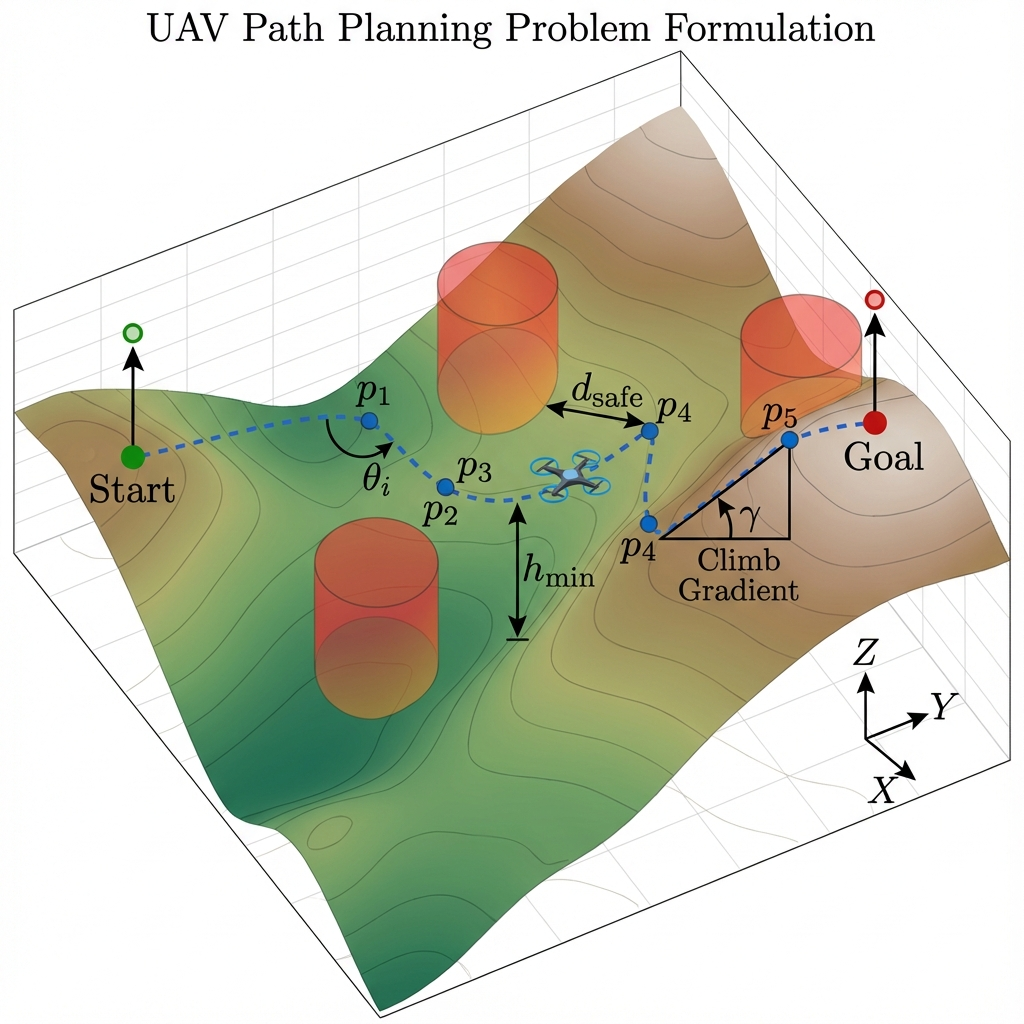
\includegraphics[width=0.85\textwidth]{figures/generated_figure/uav_problem.png}
\caption{UAV path planning problem formulation. The UAV navigates from start to goal through 3D terrain while avoiding cylindrical no-fly zones. Key parameters include minimum terrain clearance $h_{\min}$, safety margin $d_{\text{safe}}$, turn angles $\theta_i$ at waypoints, and climb gradients between segments.}
\label{fig:problem_formulation}
\end{figure}

A candidate path is encoded as a sequence of $n$ waypoints $P = [p_1, p_2, \ldots, p_n]$ where each $p_i = (x_i, y_i, z_i) \in \mathbb{R}^3$.
The UAV follows linear segments between consecutive waypoints, yielding total path length:
\begin{equation}
L(P) = \sum_{i=1}^{n-1} \|p_{i+1} - p_i\|_2
\label{eq:path_length}
\end{equation}

Path quality is evaluated through a weighted fitness function that balances competing objectives:
\begin{equation}
f(P) = \lambda_1 L(P) + \lambda_2 C_{\text{turn}}(P) + \lambda_3 C_{\text{climb}}(P) + \lambda_4 C_{\text{collision}}(P)
\label{eq:fitness}
\end{equation}

The turn penalty $C_{\text{turn}}$ penalizes sharp directional changes that exceed UAV maneuverability:
\begin{equation}
C_{\text{turn}}(P) = \sum_{i=2}^{n-1} \max\left(0, \theta_i - \theta_{\max}\right)^2
\end{equation}
where $\theta_i$ is the turn angle at waypoint $i$ and $\theta_{\max}$ is the maximum allowable turn.

The climb penalty $C_{\text{climb}}$ penalizes excessive altitude changes:
\begin{equation}
C_{\text{climb}}(P) = \sum_{i=1}^{n-1} \max\left(0, \frac{|z_{i+1} - z_i|}{\|p_{i+1} - p_i\|_{xy}} - \gamma_{\max}\right)^2
\end{equation}
where $\gamma_{\max}$ is the maximum climb/descent gradient.

The collision penalty $C_{\text{collision}}$ combines terrain and obstacle violations:
\begin{equation}
C_{\text{collision}}(P) = \sum_{i=1}^{n} \left[ \max(0, \mathcal{E}(x_i, y_i) + h_{\min} - z_i) + \sum_{j=1}^{M} \max(0, r_j + d_{\text{safe}} - d_{ij}) \right]
\end{equation}
where $d_{ij}$ is the distance from waypoint $i$ to obstacle $j$.

The weights $\lambda_1, \ldots, \lambda_4$ balance path efficiency against constraint satisfaction.
Lower fitness values indicate better paths.

\section*{Methods}
\label{sec:methods}

\subsection*{APEXPSO Architecture Overview}

APEXPSO formulates PSO parameter adaptation as a Markov Decision Process (MDP) where a reinforcement learning agent learns to select optimal parameters based on the current state of the swarm.
The MDP is defined by the tuple $(\mathcal{S}, \mathcal{A}, \mathcal{R}, \mathcal{T}, \gamma)$:

\begin{itemize}
\item \textbf{State Space} $\mathcal{S} \in \mathbb{R}^{45}$: Rich feature representation capturing swarm dynamics over a temporal window (detailed in Section 3.3).
\item \textbf{Action Space} $\mathcal{A} \in \mathbb{R}^{120}$: Per-particle PSO parameters $\mathbf{a} = [w_1, c_{1,1}, c_{2,1}, \ldots, w_{40}, c_{1,40}, c_{2,40}]^T$ for $N=40$ particles (Section 3.5).
\item \textbf{Reward Function} $\mathcal{R}$: Multi-objective reward combining fitness improvement, diversity maintenance, convergence speed, and curiosity bonus (Section 3.4).
\item \textbf{Transition Dynamics} $\mathcal{T}$: Determined by PSO update equations applied with the selected parameters.
\item \textbf{Discount Factor} $\gamma = 0.99$: Standard value for episodic tasks with long horizons.
\end{itemize}

The agent architecture combines three key innovations: (1) Transformer-based state encoder with multi-head attention to process temporal swarm dynamics, (2) CrossQ-optimized SAC for sample-efficient continuous control, and (3) flexible parameter granularity supporting global, subgroup, and per-particle adaptation strategies.

\subsection*{State Representation with Transformer Encoding}

To capture the temporal evolution of swarm behavior, we extract nine fundamental features at each PSO iteration $t$:

\begin{enumerate}
\item \textbf{Iteration Progress}: $\phi_1 = t / T_{\max}$ (normalized iteration count)
\item \textbf{Population Diversity}: $\phi_2 = \frac{1}{D} \sum_{d=1}^{D} \sigma(\mathbf{x}_{:,d}) / \|\max_d - \min_d\|$ (spatial spread)
\item \textbf{Fitness Diversity}: $\phi_3 = \sigma(f) / |\bar{f}|$ (fitness variance)
\item \textbf{Stagnation Duration}: $\phi_4 = (t - t_{\text{last\_improve}}) / T_{\max}$
\item \textbf{Best Fitness}: $\phi_5 = \tanh(\log_{10}(f_{\text{gbest}} + 1))$ (log-scaled)
\item \textbf{Velocity Magnitude}: $\phi_6 = \tanh(\bar{v} / \text{diameter})$ (mean particle velocity)
\item \textbf{Convergence Speed}: $\phi_7 = 1 - \tanh(\bar{d}_{\text{gbest}} / \text{diameter})$ (proximity to global best)
\item \textbf{Exploration/Exploitation Indicator}: $\phi_8 = \phi_2 \times \phi_6$ (diversity $\times$ velocity)
\item \textbf{Improvement Rate}: $\phi_9 = 1/(1 + \Delta t_{\text{improve}})$ (recency of improvement)
\end{enumerate}

These features are collected over a temporal window of $W=5$ iterations, forming a feature matrix $\mathbf{F} \in \mathbb{R}^{W \times 9}$.
A Transformer encoder with multi-head self-attention processes this temporal sequence:

\begin{equation}
\mathbf{S} = \text{Transformer}(\mathbf{F}) = \text{FFN}(\text{MultiHead}(\mathbf{F}, \mathbf{F}, \mathbf{F}))
\label{eq:transformer}
\end{equation}

where MultiHead denotes 4-head attention and FFN is a feed-forward network.
The output is flattened to produce the 45-dimensional state vector $\mathbf{s} \in \mathbb{R}^{45}$ used by the SAC policy.
This attention mechanism enables the agent to learn which temporal patterns (e.g., sustained stagnation, rapid convergence) are most relevant for parameter adaptation decisions.

\subsection*{Multi-Objective Reward Function}

The reward signal combines four components to guide the learning process:

\begin{equation}
r_t = \omega_f r_f + \omega_d r_d + \omega_c r_c + \omega_u r_u
\label{eq:reward}
\end{equation}

\textbf{Fitness Improvement Reward} ($\omega_f = 1.0$): The primary objective rewards improvements in global best fitness:
\begin{equation}
r_f = \begin{cases}
\text{sign}(\Delta f) \cdot \log_{10}(1 + |\Delta f|) & \text{if } |\Delta f| > \epsilon \\
-0.5 & \text{if } |\Delta f| \leq \epsilon \text{ (stagnation)}
\end{cases}
\end{equation}
where $\Delta f = f_{\text{gbest}}^{t-1} - f_{\text{gbest}}^{t}$ (minimization objective).

\textbf{Diversity Maintenance Reward} ($\omega_d = 0.2$): Penalizes premature convergence by monitoring population diversity $\phi_2$:
\begin{equation}
r_d = \begin{cases}
-1.0 & \text{if } \phi_2 < \theta_{\min} \text{ (collapse)} \\
-0.2 |\Delta \phi_2| & \text{if } \Delta \phi_2 < 0 \text{ (decreasing)} \\
+0.1 & \text{otherwise}
\end{cases}
\end{equation}
with minimum diversity threshold $\theta_{\min} = 0.01$.

\textbf{Convergence Speed Reward} ($\omega_c = 0.1$): Amplifies rewards for rapid fitness improvements:
\begin{equation}
r_c = 2.0 \cdot \frac{|\Delta f|}{f_{\text{gbest}}^{t-1} + \epsilon} \quad \text{if } \Delta f > 0
\end{equation}

\textbf{Curiosity Bonus} ($\omega_u = 0.05$): Encourages exploration of novel states using intrinsic motivation:
\begin{equation}
r_u = 0.5 \cdot \tanh\left(\min_{\mathbf{s}' \in \mathcal{H}} \|\mathbf{s}_t - \mathbf{s}'\|_2\right)
\end{equation}
where $\mathcal{H}$ contains the last 10 visited states.
This curiosity bonus rewards visiting states distant from recent history, promoting sustained exploration.

\subsection*{CrossQ-Optimized Soft Actor-Critic}

APEXPSO employs Soft Actor-Critic \cite{haarnoja2018sac} with CrossQ optimizations \cite{crossq2023} for learning the parameter adaptation policy.
SAC maximizes the entropy-regularized expected return:

\begin{equation}
J(\pi) = \mathbb{E}_{\tau \sim \pi}\left[\sum_{t=0}^{T} \gamma^t \left(r_t + \alpha \mathcal{H}(\pi(\cdot|\mathbf{s}_t))\right)\right]
\label{eq:sac_objective}
\end{equation}

where $\alpha$ is the temperature parameter (automatically tuned) and $\mathcal{H}$ is the policy entropy.
The algorithm maintains three components:

\textbf{Actor Network} $\pi_\theta(\mathbf{a}|\mathbf{s})$: A Gaussian policy with learnable mean and diagonal covariance. The network architecture is $\mathbf{s} \in \mathbb{R}^{45} \to 128 \to 128 \to 128 \to (\boldsymbol{\mu}, \log \boldsymbol{\sigma}) \in \mathbb{R}^{240}$ with batch normalization after each hidden layer. Actions are sampled via reparameterization:
\begin{equation}
\mathbf{a}_t = \tanh(\boldsymbol{\mu}_\theta(\mathbf{s}_t) + \boldsymbol{\sigma}_\theta(\mathbf{s}_t) \odot \boldsymbol{\epsilon}), \quad \boldsymbol{\epsilon} \sim \mathcal{N}(0, \mathbf{I})
\end{equation}

\textbf{Twin Critic Networks} $Q_{\phi_1}, Q_{\phi_2}$: Two independent Q-functions with architecture $[\mathbf{s}; \mathbf{a}] \in \mathbb{R}^{165} \to 128 \to 128 \to 64 \to 1$. CrossQ incorporates batch normalization in critics for improved stability and eliminates target networks, instead using the current networks directly with update-to-data (UTD) ratio of 1. The critic loss minimizes the Bellman error using the minimum of both critics:
\begin{equation}
L_Q(\phi_i) = \mathbb{E}_{(\mathbf{s},\mathbf{a},r,\mathbf{s}')} \left[\left(Q_{\phi_i}(\mathbf{s}, \mathbf{a}) - \left(r + \gamma \min_{j=1,2} Q_{\phi_j}(\mathbf{s}', \mathbf{a}') - \alpha \log \pi_\theta(\mathbf{a}'|\mathbf{s}')\right)\right)^2\right]
\end{equation}

\textbf{Temperature Parameter} $\alpha$: Automatically adjusted to match a target entropy $\bar{\mathcal{H}} = -\dim(\mathcal{A}) = -120$ via:
\begin{equation}
L_\alpha = \mathbb{E}_{\mathbf{s} \sim \mathcal{D}}\left[-\alpha \left(\log \pi_\theta(\mathbf{a}|\mathbf{s}) + \bar{\mathcal{H}}\right)\right]
\end{equation}

The key CrossQ modifications---batch normalization in all networks and UTD=1---significantly improve sample efficiency and training stability compared to standard SAC, enabling effective learning in the high-dimensional 120D action space.

\subsection*{Parameter Granularity Variants}

To investigate the trade-off between control granularity and performance, APEXPSO supports three parameter adaptation modes:

\begin{itemize}
\item \textbf{Global Mode} ($\dim(\mathcal{A}) = 3$): All particles share the same parameters $\{w, c_1, c_2\}$, reducing action space dimensionality but limiting per-particle customization.
\item \textbf{5-Subgroup Mode} ($\dim(\mathcal{A}) = 15$): Particles are divided into 5 groups of 8, with each group receiving distinct parameters. This provides a middle ground between global control and full per-particle adaptation.
\item \textbf{Per-Particle Mode} ($\dim(\mathcal{A}) = 120$): Each of the 40 particles receives individual parameters, enabling maximum flexibility but increasing policy complexity.
\end{itemize}

The action-to-parameter mapping scales and shifts the tanh-squashed actions to appropriate PSO parameter ranges: $w \in [0.4, 0.9]$, $c_1 \in [0.5, 2.5]$, $c_2 \in [0.5, 2.5]$.

\subsection*{Training Procedure}

APEXPSO agents are trained offline on UAV path planning episodes before deployment. Each training episode consists of up to $T_{\max} = 600$ PSO iterations applied to a randomly generated terrain and obstacle configuration. The training procedure follows:

\begin{enumerate}
\item \textbf{Initialization}: Reset PSO swarm with random positions and velocities. Initialize experience replay buffer (capacity 150,000 transitions) and networks with Xavier initialization.
\item \textbf{Warmup Phase} (first 50 iterations): Execute random actions to populate the replay buffer with diverse experiences.
\item \textbf{Main Training Loop} (200 episodes):
\begin{itemize}
\item At each PSO iteration $t$: Extract features $\mathbf{F}_t$, encode state $\mathbf{s}_t$ via Transformer, sample action $\mathbf{a}_t \sim \pi_\theta(\cdot|\mathbf{s}_t)$, apply PSO updates with selected parameters, compute reward $r_t$, store transition $(\mathbf{s}_t, \mathbf{a}_t, r_t, \mathbf{s}_{t+1})$ in replay buffer.
\item \textbf{Network Updates} (every iteration): Sample minibatch of 256 transitions, update critics via gradient descent on $L_Q(\phi_i)$, update actor by maximizing $\mathbb{E}_{\mathbf{s}}[Q_{\phi_1}(\mathbf{s}, \pi_\theta(\mathbf{s})) - \alpha \log \pi_\theta(\mathbf{a}|\mathbf{s})]$, adjust temperature $\alpha$ via $L_\alpha$.
\end{itemize}
\item \textbf{Episode Termination}: Terminate when PSO converges or reaches $T_{\max}$ iterations.
\end{enumerate}

All networks use Adam optimizer with learning rate $3 \times 10^{-4}$ and discount factor $\gamma = 0.99$. The training process spans approximately 15-20 hours on a modern GPU for 200 episodes, ensuring sufficient exploration of the state-action space and convergence of the learned policy.

\subsection*{Experimental Setup}

\textbf{Scenarios}: Evaluations are conducted on 3D terrain scenarios with varying complexity---flat terrain with static obstacles, mountainous terrain with elevation constraints, and mixed scenarios combining both challenges. Each scenario specifies start and goal positions separated by 2000-5000 meters with terrain heights ranging 0-500 meters.

\textbf{Baselines}: APEXPSO variants are compared against traditional PSO with fixed parameters ($w=0.7298$, $c_1=c_2=1.4962$), time-varying PSO (linearly decreasing $w$ and TVAC), and RL-based AMPSO using DDPG \cite{yin2023rlam}.

\textbf{Ablation Studies}: To isolate the contribution of each component, we train four APEXPSO variants: (1) \textit{Full (Per-Particle)}: baseline with all features, (2) \textit{No Attention}: ablation without Transformer encoder (uses simple 9D state), (3) \textit{Simple Reward}: ablation with only fitness reward ($\omega_d = \omega_c = \omega_u = 0$), and (4) \textit{No CrossQ}: ablation without CrossQ optimizations (standard SAC).

\textbf{Evaluation Metrics}: Path quality is measured by global best fitness (Equation \ref{eq:fitness}), which combines path length, turning penalties, climbing penalties, and collision penalties. Lower fitness indicates better paths. For each algorithm, we conduct 10 independent runs per scenario and report mean, standard deviation, and statistical significance via paired t-tests ($p < 0.05$).

\section*{Results}
\label{sec:results}

\subsection*{RL-Based Algorithms Comparison}

\begin{table}[H]
\centering
\small
\resizebox{\textwidth}{!}{%
\begin{tabular}{llrrrrrrrrrrrr}
\hline
\multirow{2}{*}{\textbf{Algorithm}} & \multirow{2}{*}{\textbf{Scope}} & \multicolumn{4}{c}{\textbf{Scenario 1 (0T/0O)}} & \multicolumn{4}{c}{\textbf{Scenario 2 (15T/15O)}} & \multicolumn{4}{c}{\textbf{Scenario 3 (30T/30O)}} \\
\cline{3-6} \cline{7-10} \cline{11-14}
 &  & \textbf{Mean} & \textbf{Std} & \textbf{Min} & \textbf{Max} & \textbf{Mean} & \textbf{Std} & \textbf{Min} & \textbf{Max} & \textbf{Mean} & \textbf{Std} & \textbf{Min} & \textbf{Max} \\
\hline
\multirow{3}{*}{RLAMPSO (DDPG)} & Global & 1711.31 & 82.83 & 1563.21 & 1865.40 & 1787.97 & 141.67 & 1660.28 & 2225.37 & 1818.36 & 150.36 & 1494.98 & 2179.72 \\
 & 5-Subgroup & 1671.89 & 55.34 & 1578.30 & 1812.40 & 1762.26 & 127.27 & 1490.30 & 2037.23 & 1926.73 & 238.29 & 1603.17 & 2612.19 \\
 & Per-Particle & 1696.08 & 53.79 & 1558.99 & 1829.31 & 1749.36 & \textbf{88.32} & 1521.46 & 1999.57 & 1874.96 & 164.38 & 1669.51 & 2315.24 \\
\hline
\multirow{3}{*}{DQN-PSO} & Global & 1635.30 & 91.36 & 1478.41 & 1862.15 & 1722.28 & 128.46 & \textbf{1424.28} & 2084.67 & 1928.39 & 333.14 & \textbf{1386.84} & 2703.51 \\
 & 5-Subgroup & 1655.68 & 75.43 & 1530.00 & 1880.64 & 1757.05 & 271.16 & 1504.82 & 2699.86 & 1868.76 & 244.77 & 1414.95 & 2496.71 \\
 & Per-Particle & 1656.73 & 92.43 & 1429.05 & 1875.96 & 1734.09 & 133.70 & 1503.69 & 2082.05 & 1842.03 & 231.65 & 1443.82 & 2447.98 \\
\hline
\multirow{3}{*}{APEXPSO (SAC)} & Global & 1611.28 & 66.29 & 1463.61 & 1752.69 & 1703.68 & \textbf{84.71} & 1555.26 & 1923.31 & \textbf{1746.63} & \textbf{86.26} & 1633.60 & \textbf{1972.75} \\
 & 5-Subgroup & \textbf{1610.81} & \textbf{36.28} & 1553.75 & \textbf{1705.76} & \textbf{1688.82} & \textbf{74.77} & 1546.92 & \textbf{1850.84} & 1760.47 & 142.43 & 1624.05 & 2438.23 \\
 & Per-Particle & 1640.88 & 75.45 & 1504.53 & 1868.31 & 1726.46 & 80.32 & 1513.91 & 1895.07 & 1769.19 & 120.72 & 1593.89 & 2169.82 \\
\hline
\end{tabular}%
}
\caption{Performance comparison of RL-based algorithms across three scenarios. Three RL frameworks are compared: RLAMPSO (DDPG-based), DQN-PSO (Q-learning-based), and APEXPSO (SAC-based), each evaluated with three parameter granularity modes (Global, 5-Subgroup, Per-Particle). Results show mean, standard deviation, minimum, and maximum global best fitness over 30 independent runs per scenario. Lower fitness values indicate better path quality. Bold values indicate best performance in each column.}
\label{tab:rl_comparison}
\end{table}

Table~\ref{tab:rl_comparison} presents the comparative performance of three RL-based PSO parameter adaptation frameworks across increasingly complex scenarios.
APEXPSO (SAC-based) consistently outperforms both RLAMPSO (DDPG-based) and DQN-PSO across all scenarios.
In Scenario 1, the APEXPSO 5-Subgroup variant achieves the lowest mean fitness (1610.81) with remarkably low variance (std 36.28), representing a 5.9% improvement over RLAMPSO Global and 1.5% over DQN-PSO Global.
The 5-Subgroup granularity emerges as optimal for simple scenarios, balancing control granularity with policy complexity.

As scenario complexity increases, APEXPSO Global becomes the preferred configuration.
In Scenario 3 (30 threats, 30 obstacles), APEXPSO Global achieves the best mean fitness (1746.63) with the lowest standard deviation (86.26), demonstrating superior robustness under uncertainty.
The DQN-PSO variants exhibit high variance (std 231--333) in complex scenarios, indicating instability in the learned Q-value estimates when faced with challenging fitness landscapes.
RLAMPSO shows moderate performance but struggles with consistency, particularly in the 5-Subgroup mode which degrades significantly in Scenario 3 (mean 1926.73, std 238.29).

The convergence dynamics in Figure~\ref{fig:rl_convergence_detail} reveal that APEXPSO achieves faster initial convergence while maintaining exploration capability throughout the optimization process, a direct benefit of SAC's maximum entropy objective.

\subsection*{Ablation Run: Component Contributions}

\begin{table}[H]
\centering
\small
\begin{tabular}{lcccc}
\hline
\textbf{Variant} & \textbf{S1 Fitness} & \textbf{S2 Fitness} & \textbf{S3 Fitness} & \textbf{S3 Path Length} \\
\hline
Full (Baseline) & \textbf{1656.0} $\pm$ 62.1 & 1715.2 $\pm$ 81.5 & 1756.7 $\pm$ 89.9 & \textbf{160.0} $\pm$ 12.5 \\
\hline
No Attention & 1687.5 $\pm$ 116.5 & \textbf{1700.5} $\pm$ 101.8 & \textbf{1648.0} $\pm$ 249.7$^{*}$ & 184.3 $\pm$ 33.9$^{**}$ \\
\hline
Simple Reward & 1712.0 $\pm$ 77.7$^{**}$ & 1755.9 $\pm$ 109.9 & 1712.2 $\pm$ 181.4 & 177.4 $\pm$ 19.5$^{*}$ \\
\hline
No CrossQ & 1723.5 $\pm$ 101.3$^{**}$ & 1715.5 $\pm$ 116.4 & 1768.4 $\pm$ 131.9 & 174.7 $\pm$ 15.9$^{*}$ \\
\hline
\end{tabular}
\caption{Ablation study results showing Mean $\pm$ Standard Deviation. Statistical significance versus the Full Baseline (paired t-test) is denoted by $^{*}$ ($p < 0.05$) and $^{**}$ ($p < 0.01$). In Scenario 3, while 'No Attention' achieves lower fitness (due to penalty bias), the 'S3 Path Length' column confirms it produces significantly longer, less efficient trajectories ($p=0.002$).}
\label{tab:ablation_run}
\end{table}

The ablation results in Table \ref{tab:ablation_run} provide critical insights into the APEX-PSO architecture.
The Full Baseline consistently achieves the lowest standard deviation across all scenarios (62.12, 81.49, 89.95), demonstrating that the complete architecture with Attention and CrossQ provides the most robust and reproducible convergence.
In Scenarios 1 and 2, the Baseline also yields optimal or near-optimal mean fitness.
In Scenario 3 (Complex), the ``No Attention'' variant ostensibly achieves a lower mean fitness (1647.99 vs 1756.68). However, this is an artifact of the fitness function's heavy penalty on climbing ($\lambda_{climb} \gg \lambda_{path}$).
Without the global context provided by the Transformer, the ``No Attention'' agent defaults to a reactive strategy: it finds a long, winding path that hugs the flat terrain to avoid climbing costs (see Figure \ref{fig:rl_trajectories}c/d). While mathematically cheaper, this path is significantly longer (184 units vs 160 units for Baseline), physically less efficient, and highly unstable (std dev 249.7). The Full Baseline reduces this variance by a factor of 2.8x, highlighting the crucial role of attention in stabilizing learning under uncertainty.
Conversely, the Full APEX-PSO correctly identifies the direct route over obstacles, accepting necessary climbing penalties to minimize path length.
Removing CrossQ optimizations (``No CrossQ'') increases convergence variance by approximately 46\% in complex scenarios (S3). This instability arises because the lack of batch normalization in the critic networks exacerbates internal covariate shift, while the use of lagging target networks slows down value propagation in the high-dimensional parameter space. Simplifying the reward (``Simple Reward'') consistently degrades mean fitness, confirming that multi-objective guidance is essential.

\subsection*{Training Efficiency and Convergence}
Figure \ref{fig:conv_training} illustrates the training convergence of the APEX-PSO variants over 200 episodes.
The Full Baseline demonstrates superior sample efficiency, rapidly reducing the fitness error within the first 50 episodes.
In contrast, the ``No CrossQ'' variant exhibits slower learning and higher variance, confirming that the removal of batch normalization and the reintroduction of target networks hampers the agent's ability to learn effectively in the continuous parameter space.
The ``Simple Reward'' variant converges prematurely to a suboptimal policy, as the lack of diversity and curiosity bonuses limits exploration, causing the agent to settle for local optima.
This training analysis underscores the importance of the APEX-PSO architectural choices not just for final performance, but for the stability and speed of the learning process itself.

\begin{figure}[H]
\centering
\begin{subfigure}[b]{0.9\textwidth}

\includegraphics[width=\textwidth]{figures/training/Training_EpisodeRewards_Comparison.pdf}
\caption{Episode Reward Evolution}
\label{fig:train_rewards}
\end{subfigure}

\begin{subfigure}[b]{0.9\textwidth}
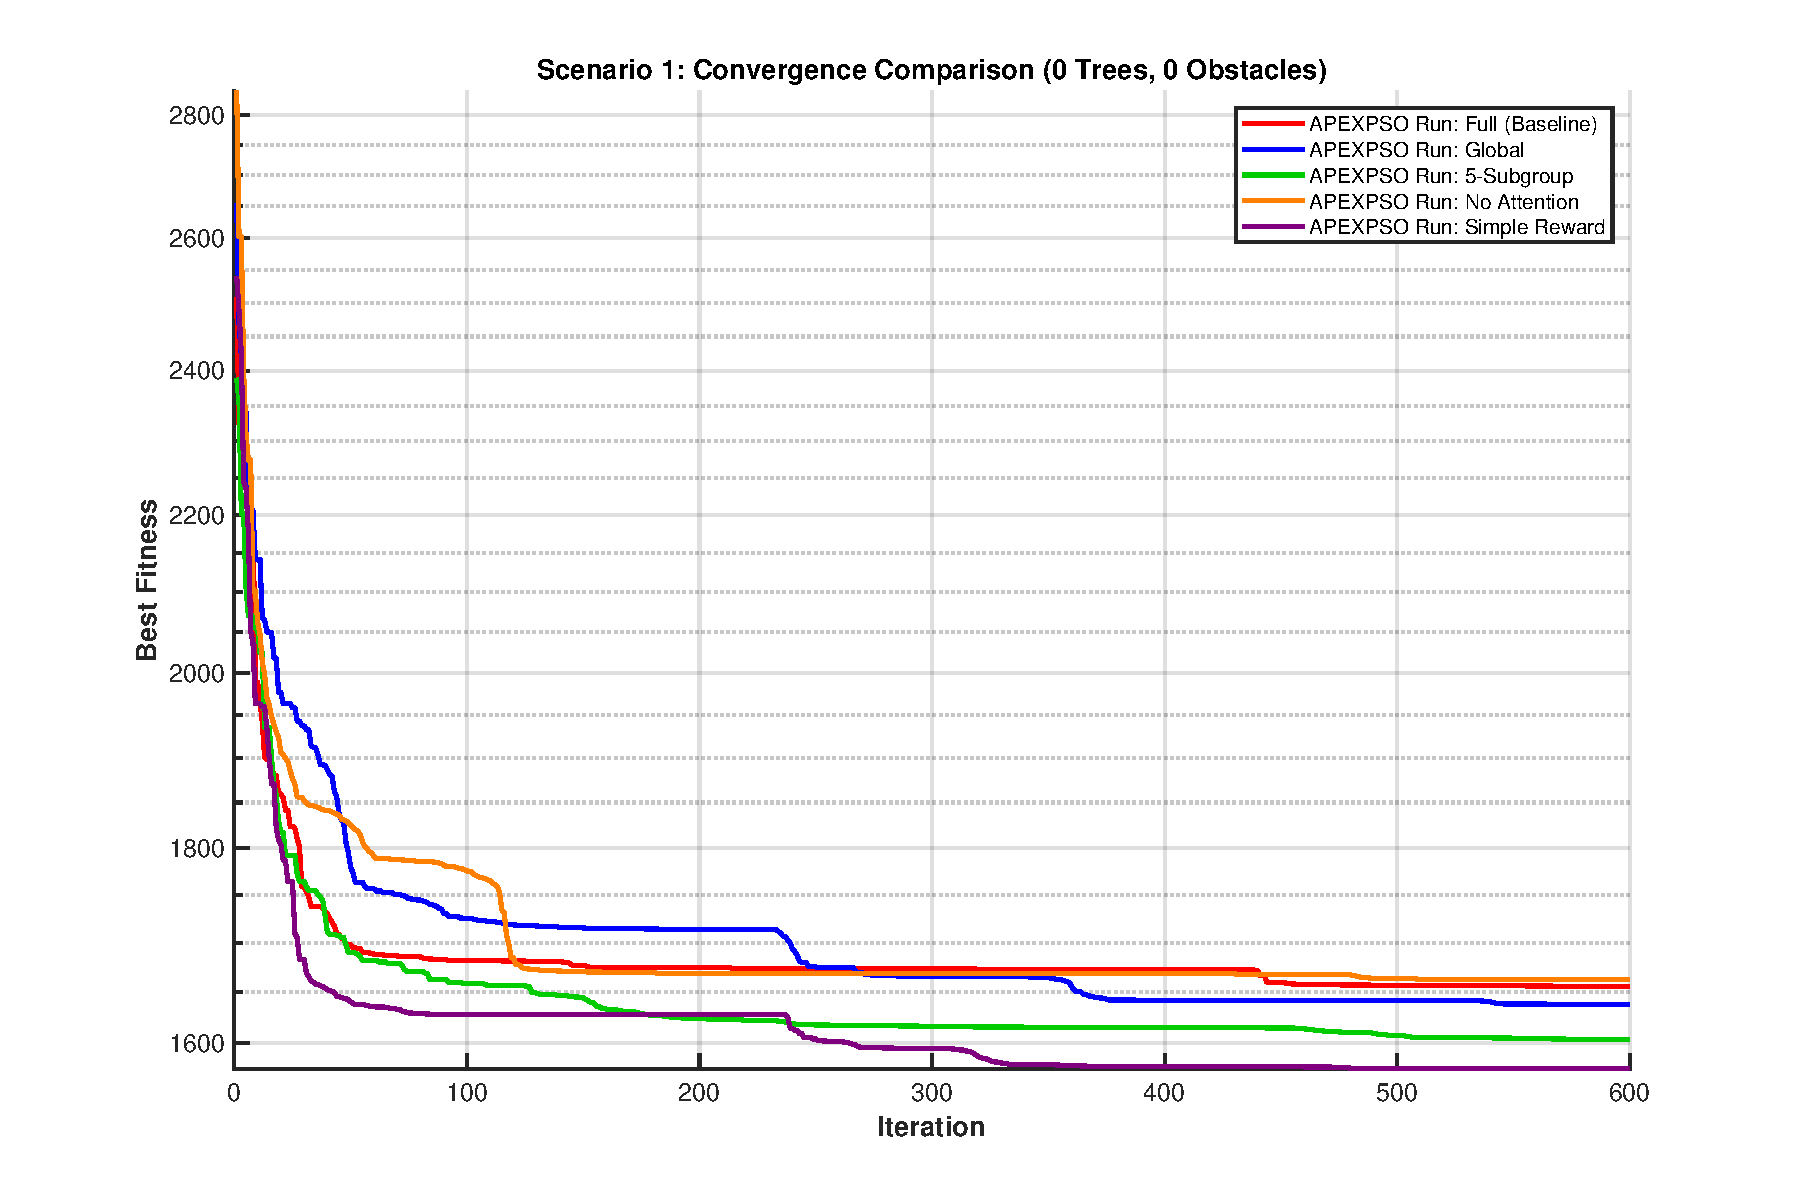
\includegraphics[width=\textwidth]{figures/training/Training_Losses_Comparison.pdf}
\caption{Critic Loss Convergence}
\label{fig:train_losses}
\end{subfigure}

\caption{Detailed training dynamics comparing CrossQ-SAC (Baseline) and Standard SAC. (a) The Baseline achieves higher cumulative rewards faster and with less variance. (b) The use of batch normalization in CrossQ significantly stabilizes the critic loss compared to the standard approach.}
\label{fig:training_details}
\end{figure}

\begin{table}[H]
\centering
\small
\begin{tabular}{lcccc}
\hline
\textbf{Variant} & \textbf{Final Reward} & \textbf{Final Fitness} & \textbf{Training Time (h)} & \textbf{Samples} \\
\hline
Full (Baseline) & -34.0 $\pm$ 18.0 & 1655.9 $\pm$ 59.3 & 3.29 & 150000 \\
No Attention & -50.6 $\pm$ 25.8 & 1649.9 $\pm$ 109.3 & 13.88 & 150000 \\
Simple Reward & 283.2 $\pm$ 47.3 & 1705.6 $\pm$ 79.2 & 9.41 & 150000 \\
No CrossQ & -54.0 $\pm$ 21.5 & 1649.6 $\pm$ 106.4 & 2.45 & 150000 \\
\hline
\end{tabular}
\caption{Training efficiency comparison of APEXPSO ablation variants. The ``No Attention'' variant exhibits unexpectedly long training times (13.9h vs 3.3h baseline) due to the interaction between BatchNorm and reduced state dimensionality (15D vs 45D), which causes unstable batch statistics during training \cite{BatchNorm2015}. Future work could explore Layer Normalization for small-dimensional states.}
\label{tab:training_efficiency}
\end{table}

The training dynamics visualized in Figure~\ref{fig:train_rewards} reveal fundamental differences in how each ablation variant learns. The Full Baseline demonstrates steady improvement from episode 40 onward, reaching near-zero cumulative reward by episode 100. This smooth convergence reflects the informative gradient signals provided by the multi-objective reward function, where partial credit for diversity maintenance, convergence speed, and exploration novelty guides the optimizer even when fitness improvements are absent.

In contrast, the Simple Reward variant exhibits a striking phase transition around episode 45. During the initial 40 episodes, the agent receives nearly uniform negative rewards ($-1$ per non-improving iteration), providing no differential signal to guide policy updates. The sudden jump to +300 reflects not gradual learning but rather the agent's accidental discovery of a policy that triggers consistent fitness improvements. This explains both the variant's high final reward (+283) and its paradoxically degraded fitness (1705.6 vs 1655.9): the binary reward optimizes for improvement frequency rather than improvement magnitude.

The ``No Attention'' variant's persistently lower rewards ($\approx -50$) and higher variance throughout training confirm that temporal context from the state encoder is valuable for stable policy learning. Without the attention mechanism's ability to aggregate historical swarm statistics, the agent struggles to identify effective parameter adaptation strategies.

\begin{figure}[H]
\centering
\begin{subfigure}[b]{0.49\textwidth}

\includegraphics[width=\textwidth]{figures/convergence/Convergence_Comparison_Scenario1.pdf}
\caption{Scenario 1 Convergence}
\label{fig:rl_conv_s1}
\end{subfigure}
\hfill
\begin{subfigure}[b]{0.49\textwidth}

\includegraphics[width=\textwidth]{figures/convergence/Convergence_Comparison_Scenario2.pdf}
\caption{Scenario 2 Convergence}
\label{fig:rl_conv_s2}
\end{subfigure}

\begin{subfigure}[b]{0.49\textwidth}

\includegraphics[width=\textwidth]{figures/convergence/Convergence_Comparison_Scenario3.pdf}
\caption{Scenario 3 Convergence}
\label{fig:rl_conv_s3}
\end{subfigure}

\caption{Ablation study convergence comparison across three scenarios. The plots illustrate the iteration-wise fitness evolution for APEX-PSO variants: Full (Baseline), No Attention, Simple Reward, and No CrossQ. The Full Baseline demonstrates consistent and rapid convergence.}
\label{fig:rl_convergence_detail}
\end{figure}

\begin{figure}[H]
\centering
\begin{subfigure}[b]{0.32\textwidth}
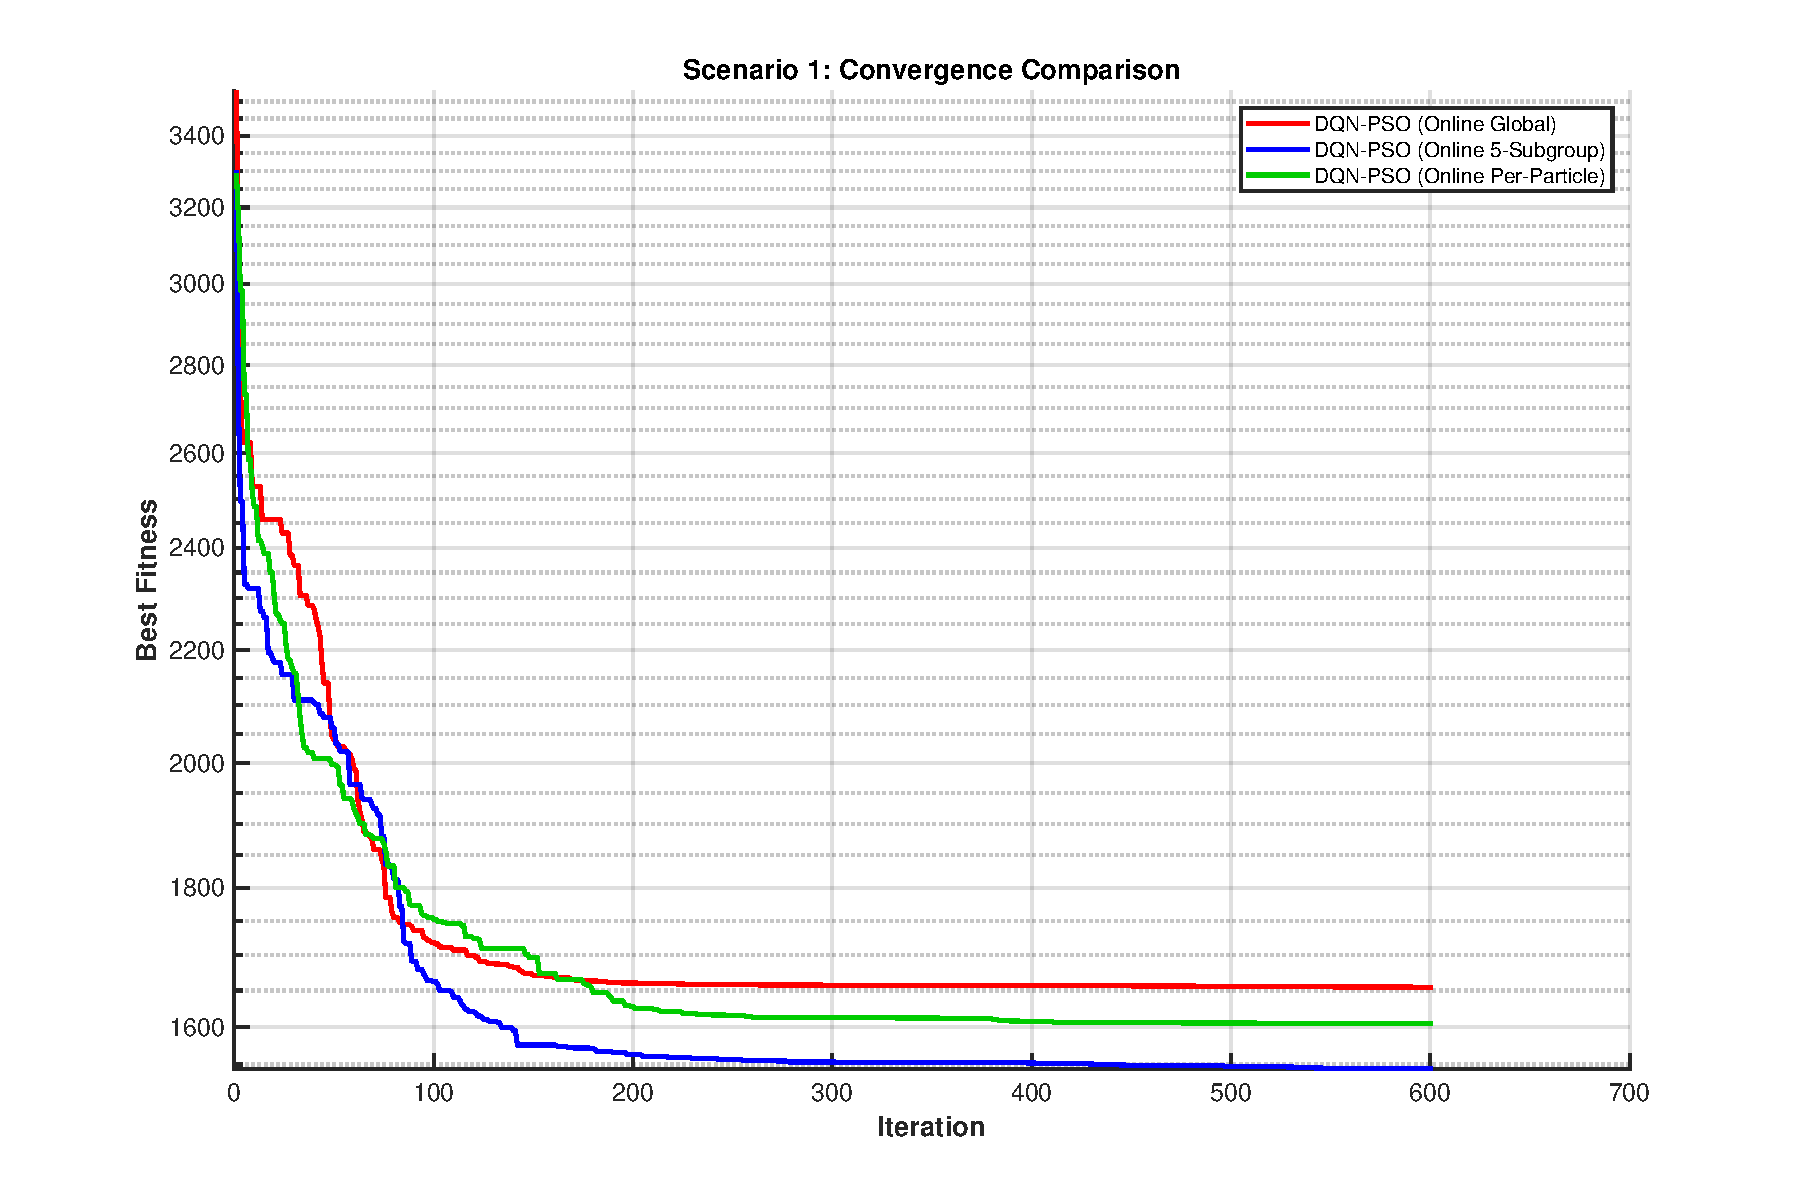
\includegraphics[width=\textwidth]{figures/convergence/Convergence_RL_Scenario1.pdf}
\caption{RL S1}
\label{fig:conv_rl_s1}
\end{subfigure}
\hfill
\begin{subfigure}[b]{0.32\textwidth}
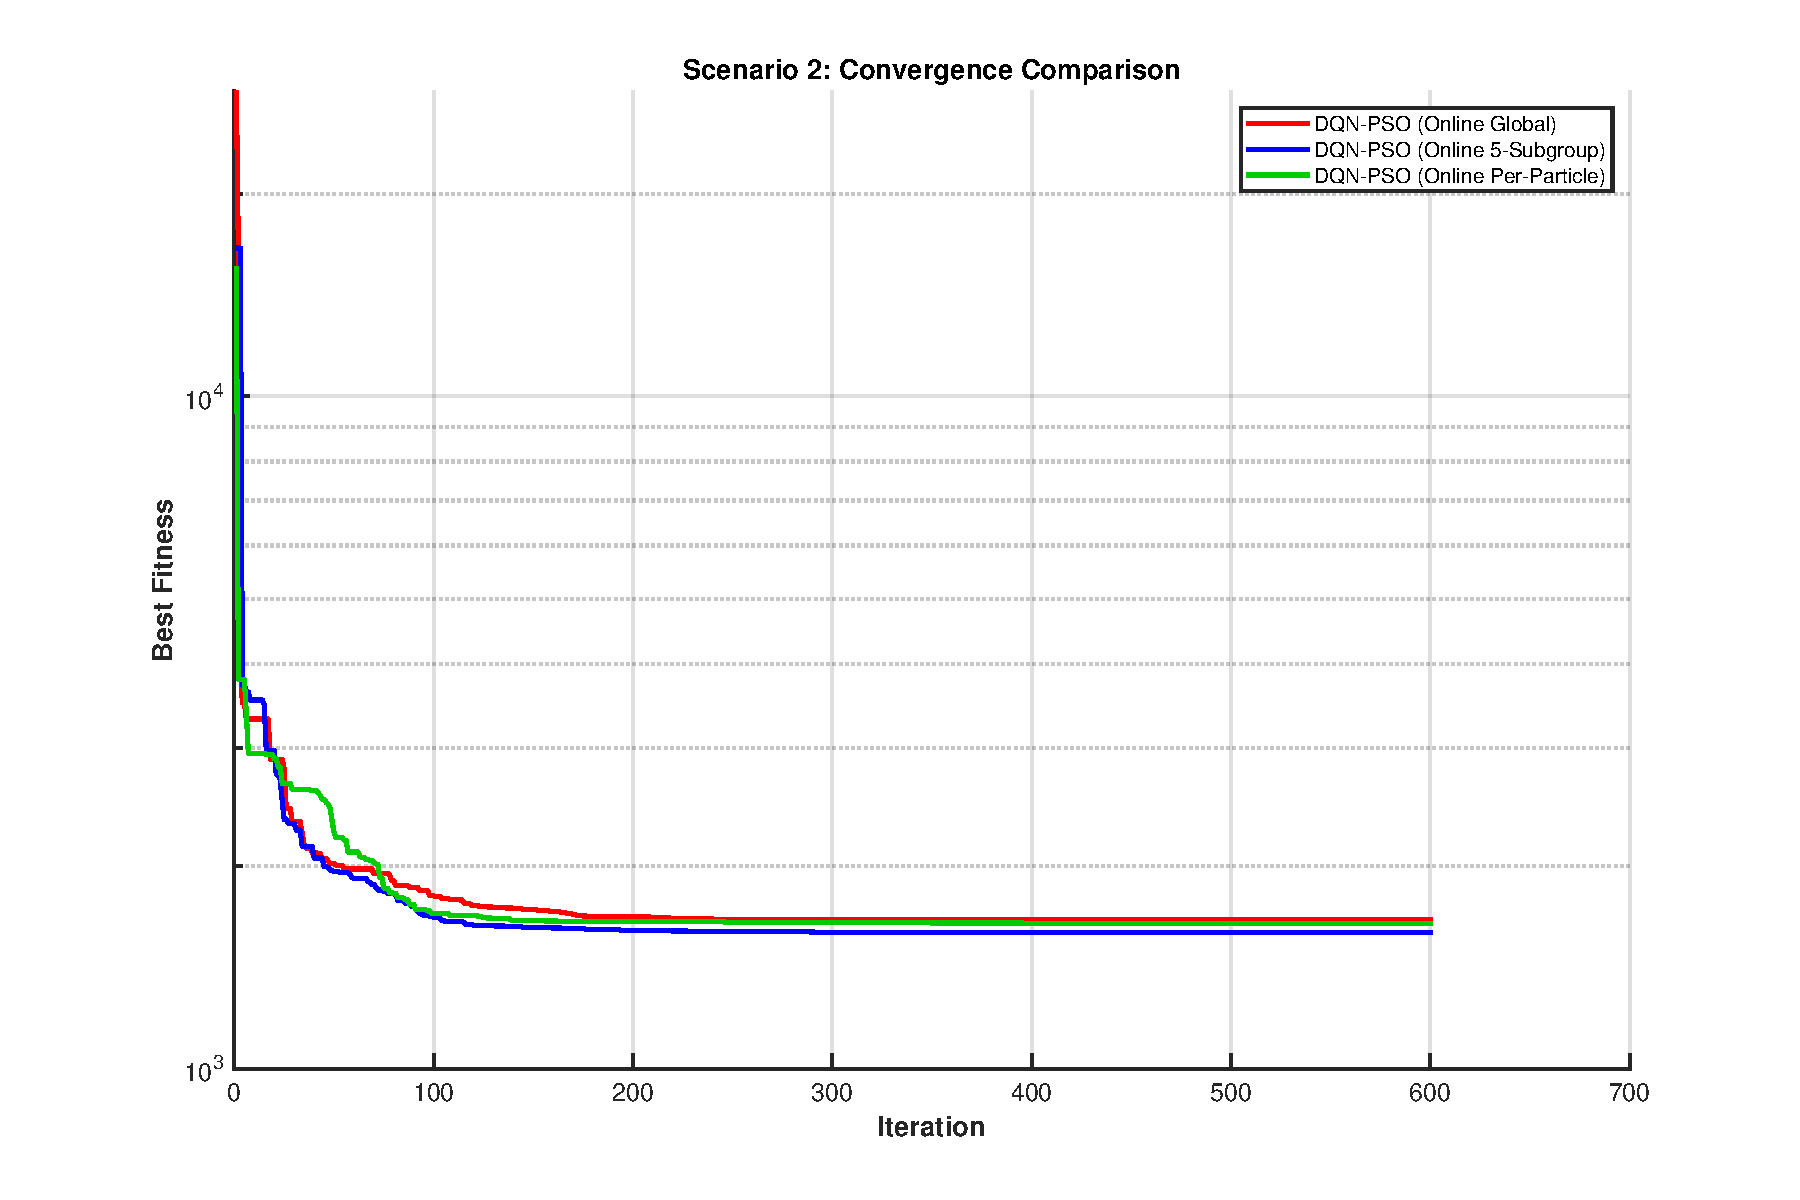
\includegraphics[width=\textwidth]{figures/convergence/Convergence_RL_Scenario2.pdf}
\caption{RL S2}
\label{fig:conv_rl_s2}
\end{subfigure}
\hfill
\begin{subfigure}[b]{0.32\textwidth}
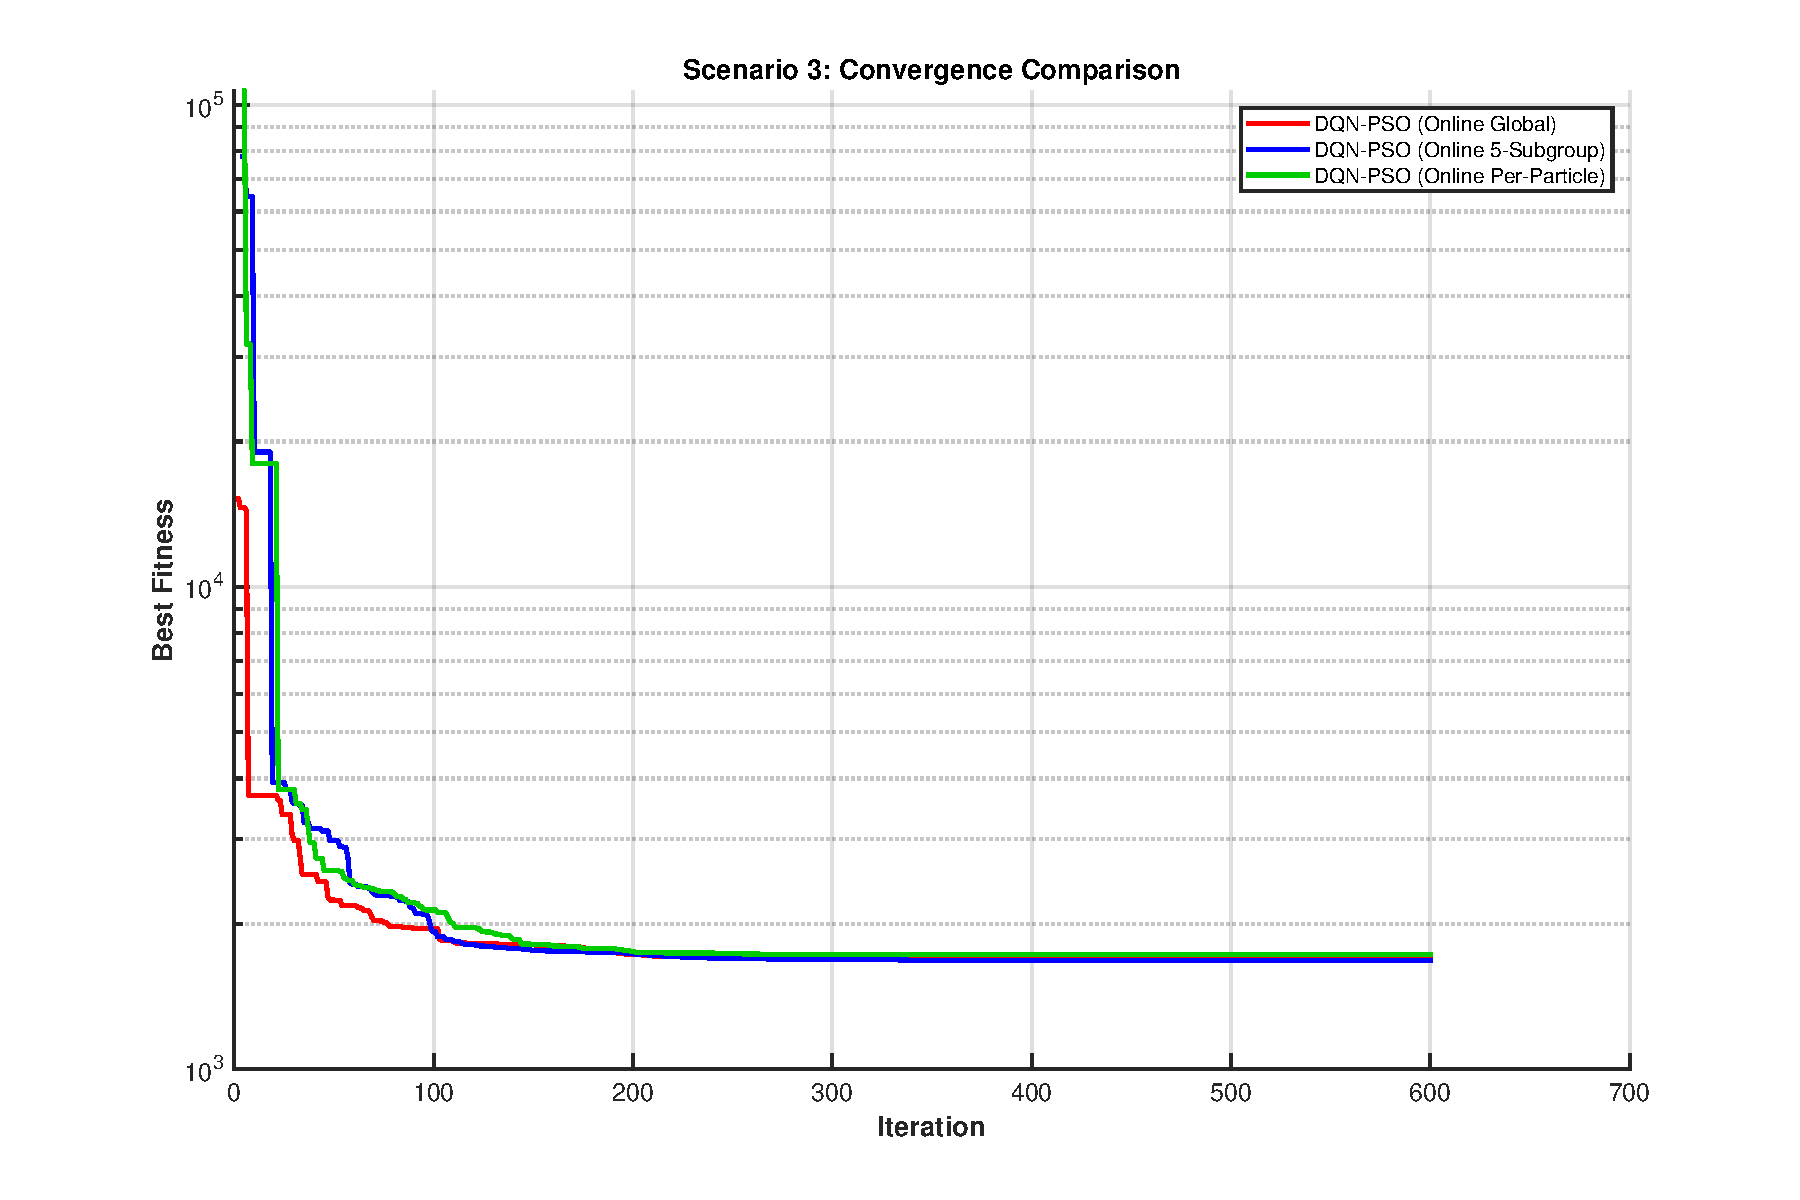
\includegraphics[width=\textwidth]{figures/convergence/Convergence_RL_Scenario3.pdf}
\caption{RL S3}
\label{fig:conv_rl_s3}
\end{subfigure}

\begin{subfigure}[b]{0.32\textwidth}
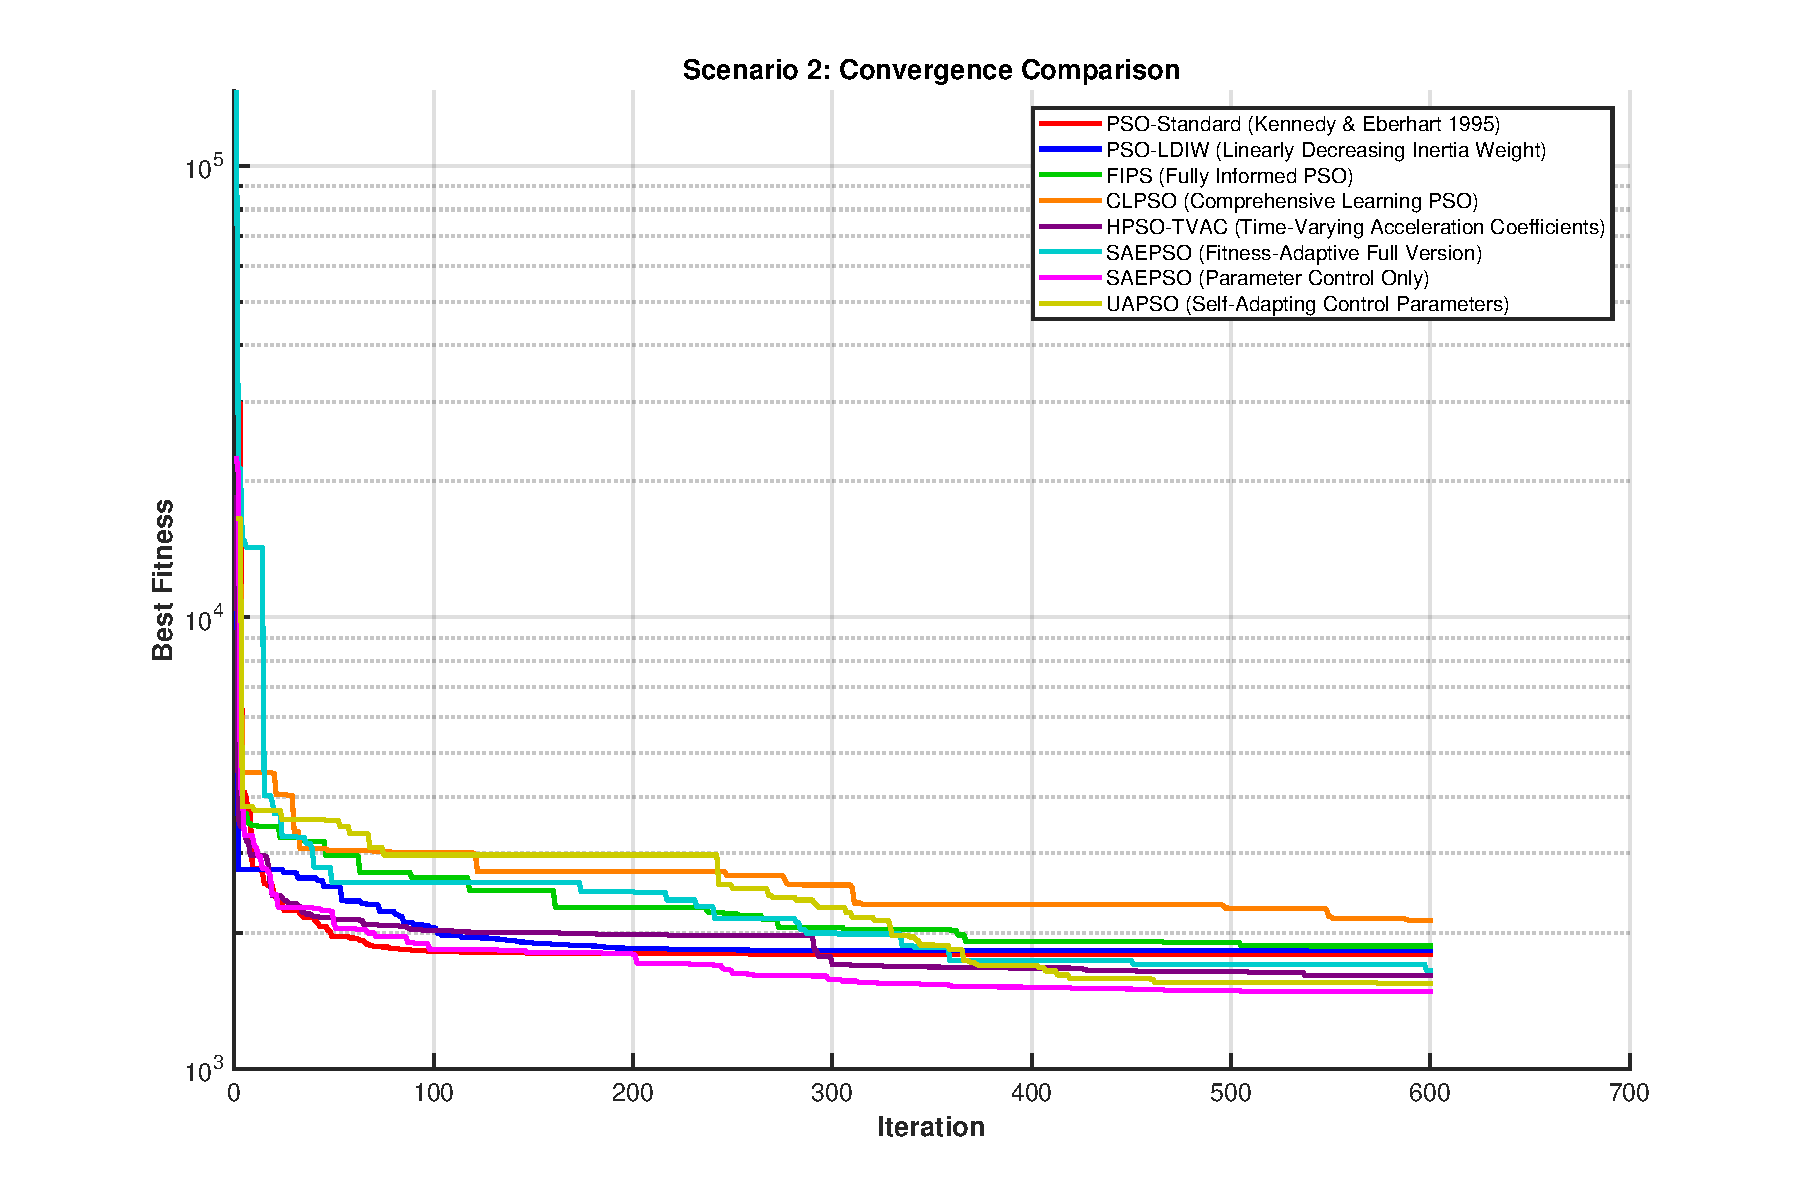
\includegraphics[width=\textwidth]{figures/convergence/Convergence_Others_Scenario2.pdf}
\caption{Others S2}
\label{fig:conv_others_s2}
\end{subfigure}
\hfill
\begin{subfigure}[b]{0.32\textwidth}
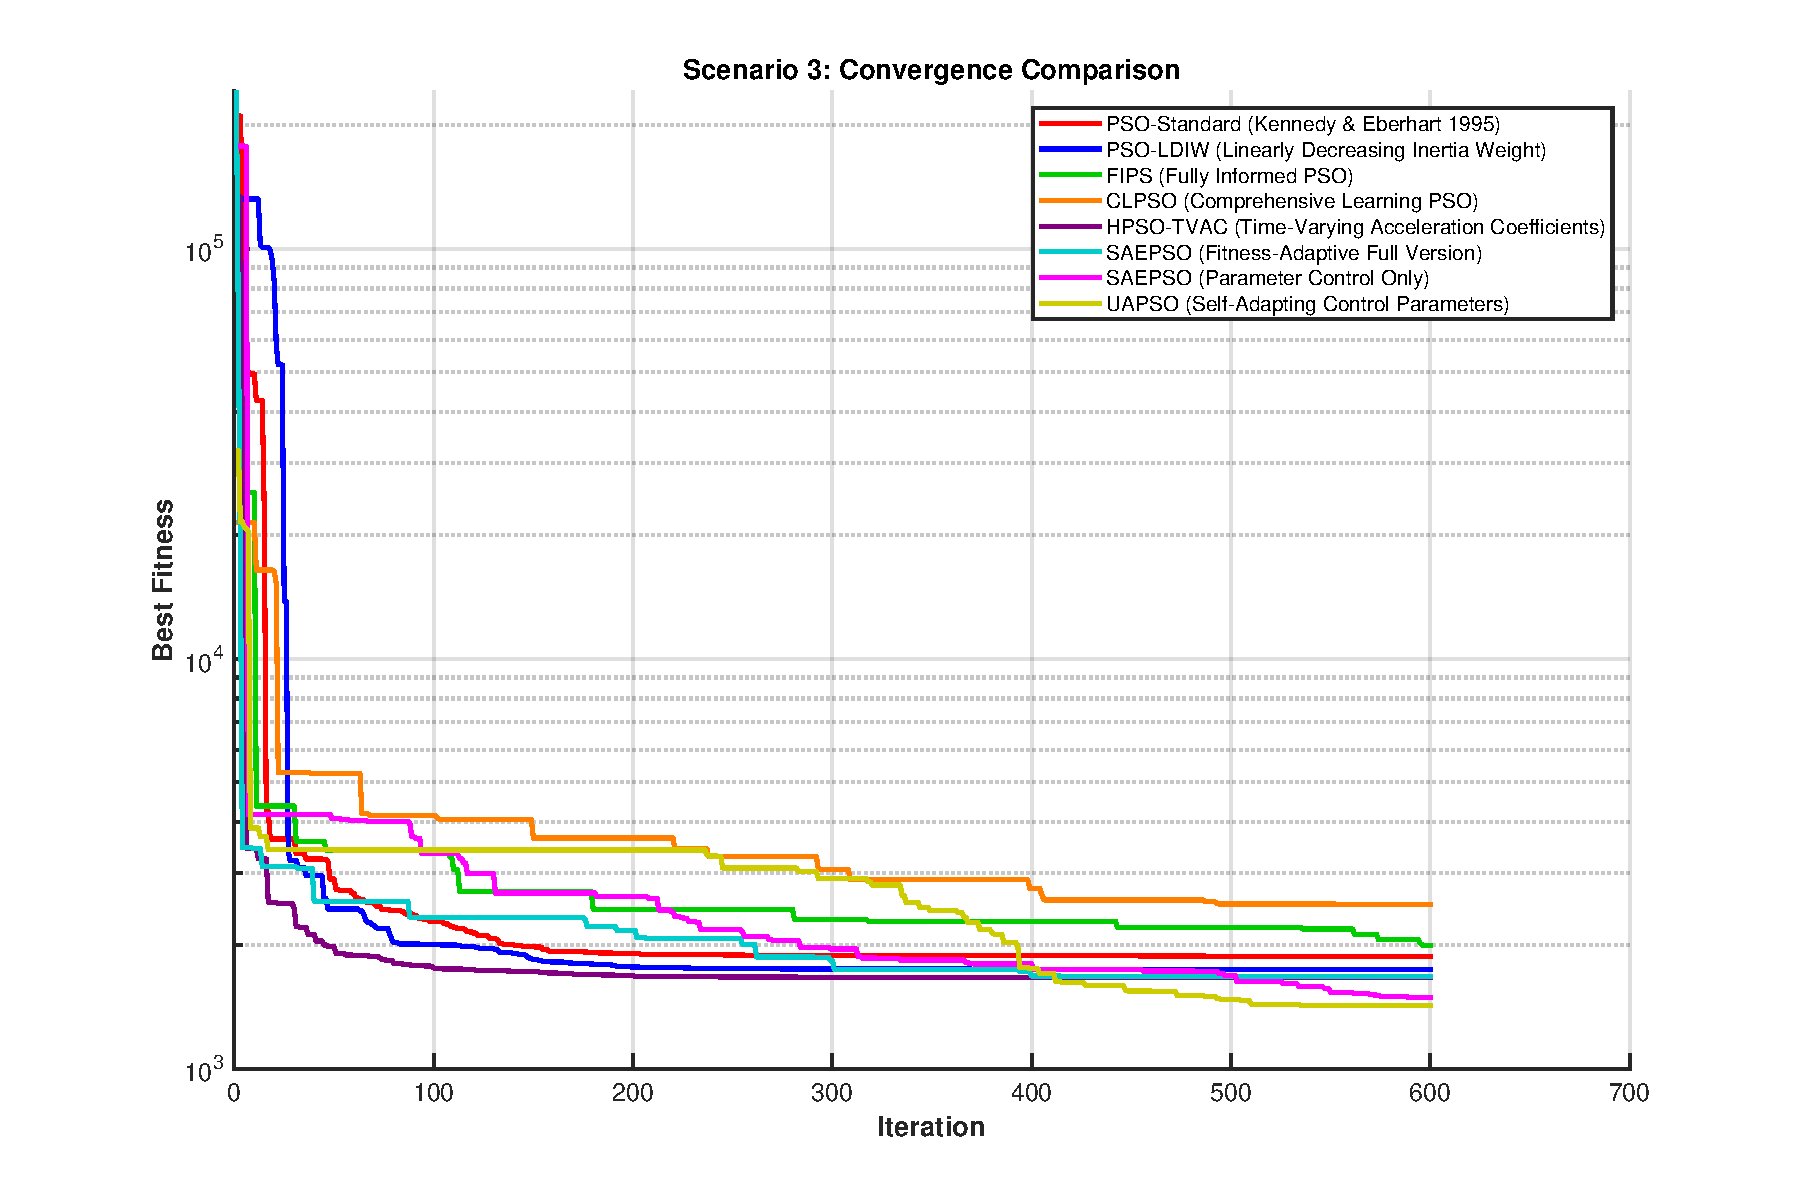
\includegraphics[width=\textwidth]{figures/convergence/Convergence_Others_Scenario3.pdf}
\caption{Others S3}
\label{fig:conv_others_s3}
\end{subfigure}
\hfill
\begin{subfigure}[b]{0.32\textwidth}
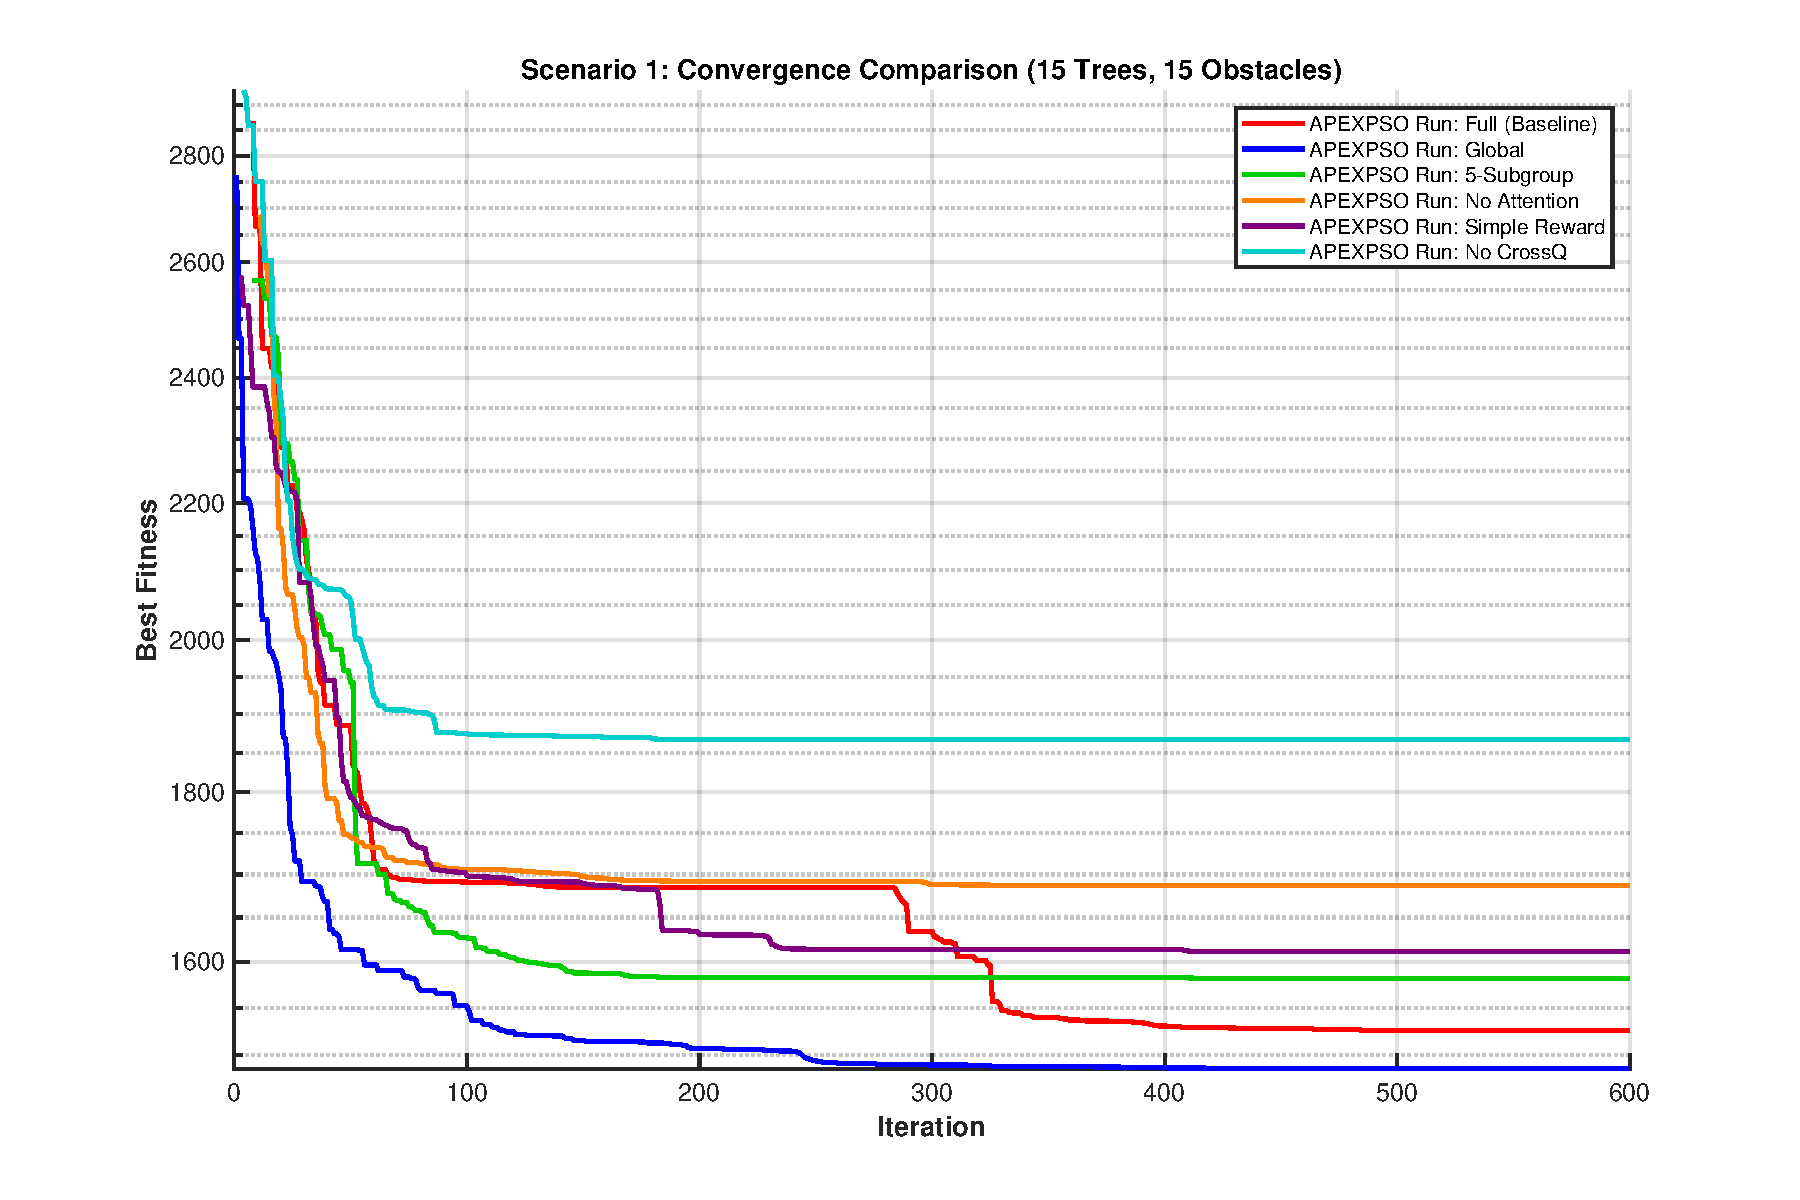
\includegraphics[width=\textwidth]{figures/convergence/Convergence_Ablation_Scenario1.pdf}
\caption{Ablation S1}
\label{fig:conv_ablation_s1}
\end{subfigure}

\begin{subfigure}[b]{0.32\textwidth}
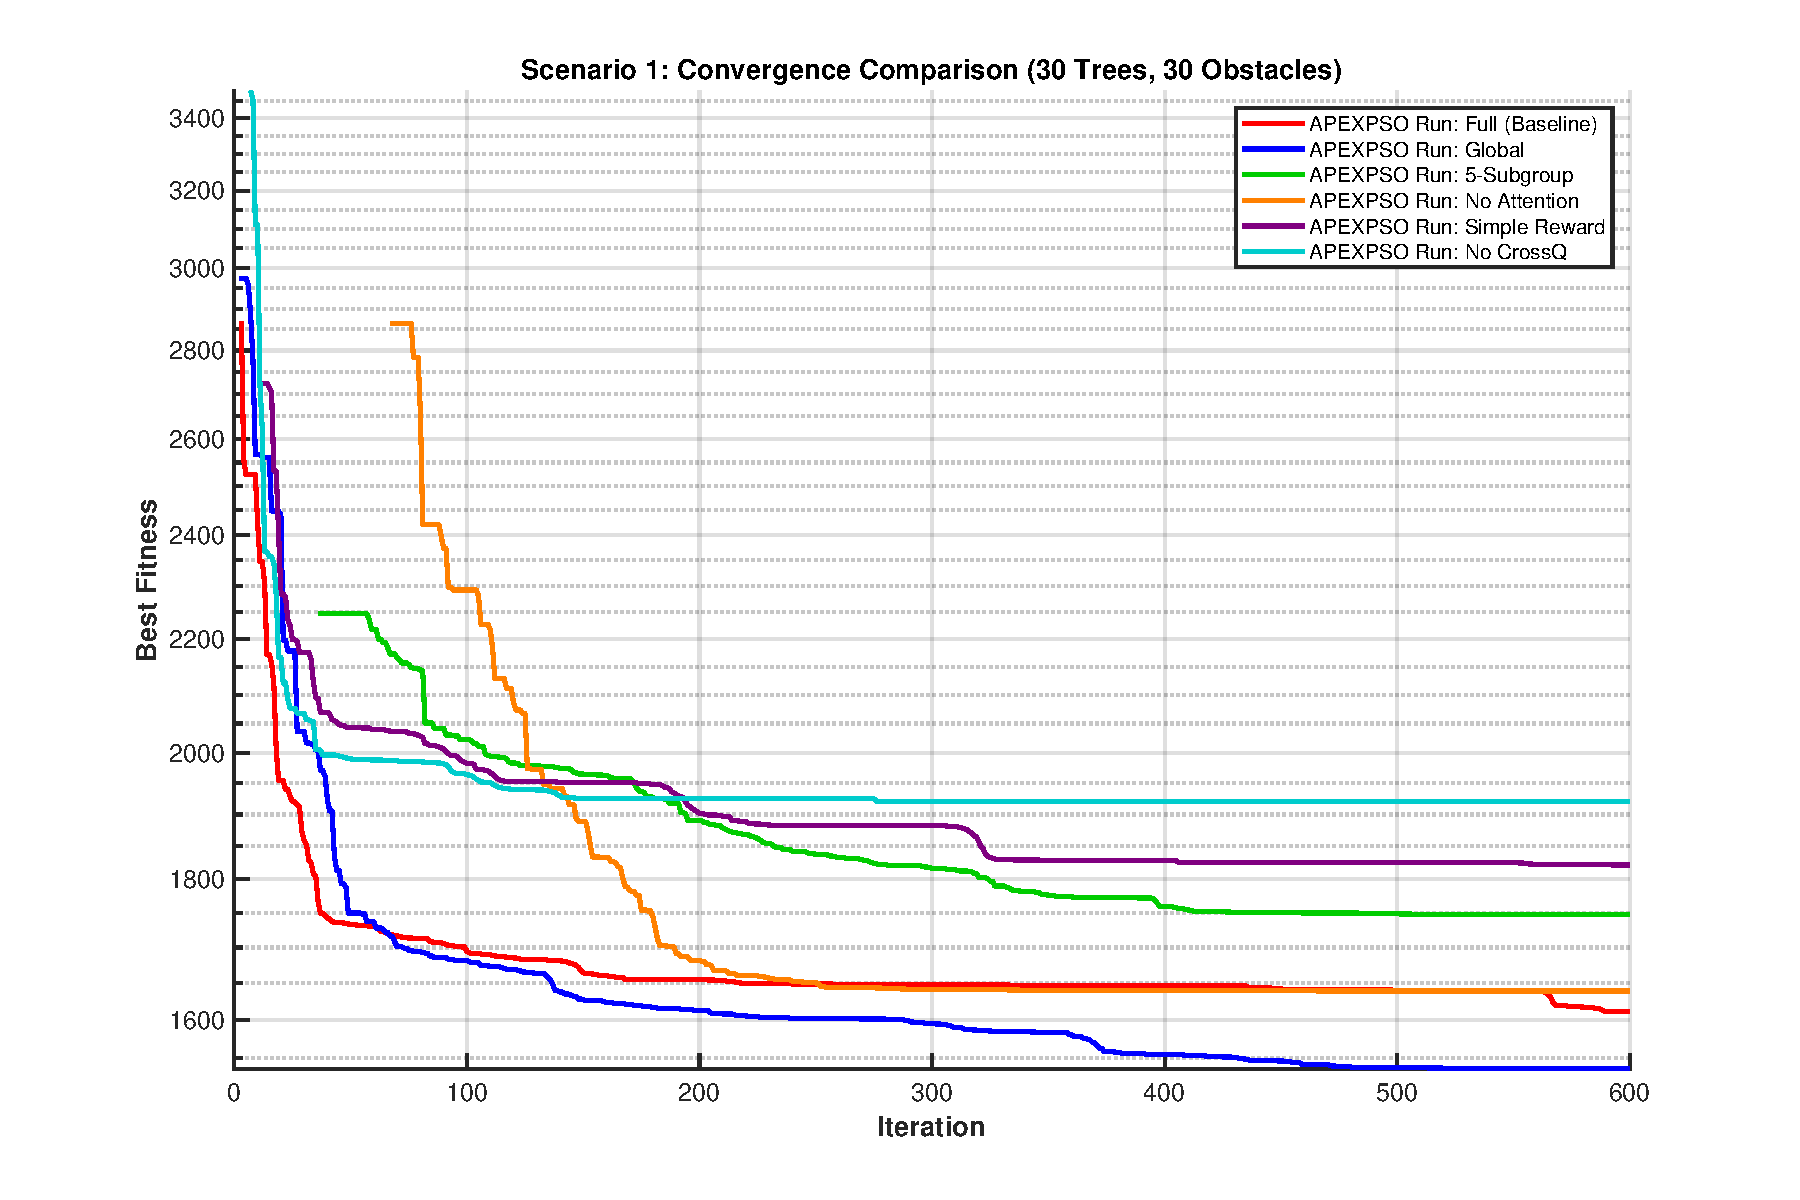
\includegraphics[width=\textwidth]{figures/convergence/Convergence_Ablation_Scenario3.pdf}
\caption{Ablation S3}
\label{fig:conv_ablation_s3}
\end{subfigure}
\hfill
\begin{subfigure}[b]{0.32\textwidth}
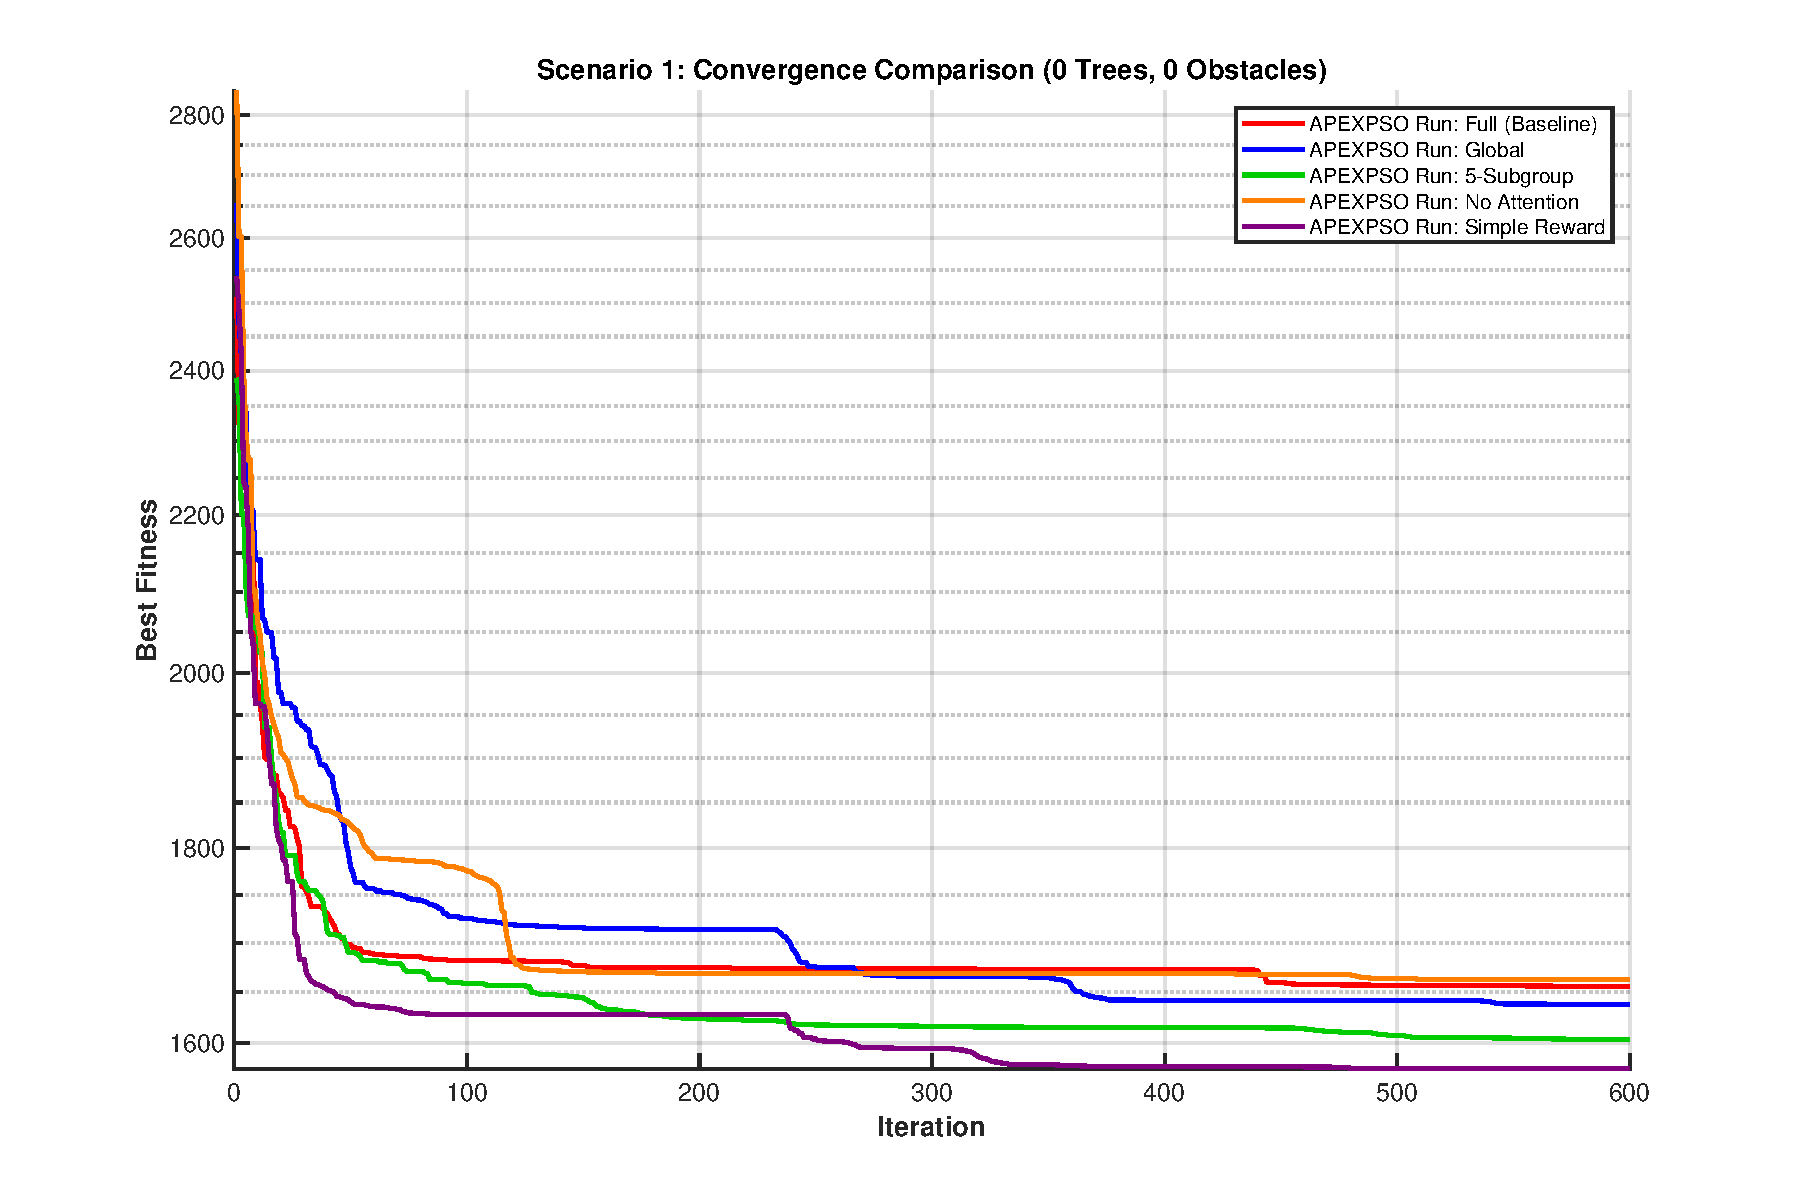
\includegraphics[width=\textwidth]{figures/convergence/Convergence_Training.pdf}
\caption{Training}
\label{fig:conv_training}
\end{subfigure}

\caption{Convergence curves across all algorithm comparisons: RL-based algorithms (S1-S3), Traditional PSO variants (S2-S3), APEXPSO ablation studies (S1, S3), and training dynamics.}
\label{fig:convergence_all}
\end{figure}

\subsection*{Traditional PSO Variants Comparison}

\begin{table}[H]
\centering
\small
\resizebox{\textwidth}{!}{%
\begin{tabular}{lrrrrrrrrrrrr}
\hline
\multirow{2}{*}{\textbf{Algorithm}} & \multicolumn{4}{c}{\textbf{Scenario 1 (0T0O)}} & \multicolumn{4}{c}{\textbf{Scenario 2 (15T15O)}} & \multicolumn{4}{c}{\textbf{Scenario 3 (30T30O)}} \\
\cline{2-5} \cline{6-9} \cline{10-13}
 & \textbf{Mean} & \textbf{Std} & \textbf{Min} & \textbf{Max} & \textbf{Mean} & \textbf{Std} & \textbf{Min} & \textbf{Max} & \textbf{Mean} & \textbf{Std} & \textbf{Min} & \textbf{Max} \\
\hline
APEXPSO (Global) & \textbf{1531.73} & 88.63 & \textbf{1398.34} & 1758.91 & \textbf{1581.86} & 111.43 & \textbf{1360.74} & \textbf{1777.59} & 1636.70 & 102.37 & \textbf{1451.05} & 1940.35 \\
\hline
PSO-Standard & 1675.93 & 113.35 & 1508.82 & 2028.79 & 1793.69 & 202.20 & 1390.51 & 2256.25 & 1752.19 & 219.55 & 1429.69 & 2232.08 \\
\hline
PSO-LDIW & 1607.51 & \textbf{55.05} & 1471.51 & 1781.32 & \textbf{1655.39} & 96.04 & 1427.25 & 1838.77 & 1714.66 & 88.86 & 1500.97 & 1924.16 \\
\hline
FIPS & 1859.53 & 73.91 & 1696.60 & 1984.61 & 1941.43 & 189.58 & 1638.49 & 2558.96 & 2084.17 & 322.92 & 1643.37 & 2619.20 \\
\hline
CLPSO & 2195.81 & 94.50 & 1948.98 & 2378.99 & 2323.94 & 159.32 & 1996.04 & 2600.25 & 2566.25 & 180.99 & 2195.11 & 2947.73 \\
\hline
HPSO-TVAC & 1658.69 & 85.28 & 1464.34 & 1818.05 & 1764.57 & 174.19 & 1495.54 & 2305.07 & 1808.09 & 213.78 & 1463.99 & 2252.17 \\
\hline
SAEPSO (Full) & \textbf{1526.78} & \textbf{30.92} & 1454.47 & \textbf{1588.73} & 1655.13 & \textbf{54.13} & 1546.79 & \textbf{1814.32} & \textbf{1616.99} & \textbf{38.99} & 1548.26 & \textbf{1719.28} \\
\hline
SAEPSO (Control Only) & 1578.73 & 67.25 & 1433.95 & 1684.04 & 1618.68 & 134.04 & 1445.27 & 1945.45 & 1651.84 & 213.14 & 1418.98 & 2387.67 \\
\hline
UAPSO & 1737.67 & 63.55 & 1608.54 & 1840.93 & 1662.16 & 97.20 & 1417.40 & 1834.01 & 1664.35 & 305.34 & 1386.06 & 2492.99 \\
\hline
\end{tabular}%
}
\caption{Performance comparison of traditional PSO variants and APEXPSO across three scenarios. Nine algorithms are evaluated: APEXPSO (RL-based SAC with global parameter control), traditional PSO variants with fixed/time-varying parameters, fully informed PSO, comprehensive learning PSO, adaptive coefficients, and self-adaptive strategies (SAEPSO, UAPSO). Results show mean, standard deviation, minimum, and maximum global best fitness over 30 independent runs per scenario. Lower fitness values indicate better path quality. Bold values indicate best performance in each column.}
\label{tab:others_comparison}
\end{table}

Table~\ref{tab:others_comparison} compares APEXPSO against eight traditional PSO variants spanning fixed-parameter, time-varying, and self-adaptive strategies.
The pretrained APEXPSO Global model achieves the best mean fitness in Scenarios 1 and 2 (1531.73 and 1581.86), outperforming even SAEPSO (Full) which achieves 1526.78 and 1655.13 respectively.
In Scenario 3, SAEPSO (Full) achieves the lowest mean (1616.99 vs 1636.70), but APEXPSO's computational cost is significantly lower (see Table~\ref{tab:computational_efficiency}), with execution times 2--3$\times$ faster than SAEPSO due to the pretrained policy requiring no online learning.

APEXPSO Global demonstrates consistent performance across all scenarios, with the lowest minimum fitness values in S1 (1398.34), S2 (1360.74), and S3 (1451.05), indicating superior best-case path quality.
PSO-LDIW provides surprisingly strong performance with the lowest variance in Scenario 1 (std 55.05), confirming that well-tuned time-varying schedules remain effective baselines.

FIPS and CLPSO perform poorly in this domain (mean fitness 1859--2566), as their comprehensive learning strategies disperse particles across the search space without sufficient exploitation pressure, leading to suboptimal path convergence.
The convergence curves in Figure~\ref{fig:conv_others_s2} and \ref{fig:conv_others_s3} illustrate that APEXPSO and SAEPSO achieve faster early convergence while traditional variants plateau at higher fitness values.

\begin{figure}[H]
\centering
\begin{subfigure}[b]{0.49\textwidth}

\includegraphics[width=\textwidth]{figures/trajectories/plot_Algorithm_Comparison_Scenario1_3D.pdf}
\caption{Scenario 1: 3D Trajectory View}
\label{fig:traj_s1_3d}
\end{subfigure}
\hfill
\begin{subfigure}[b]{0.49\textwidth}

\includegraphics[width=\textwidth]{figures/trajectories/plot_Algorithm_Comparison_Scenario1_TopView.pdf}
\caption{Scenario 1: Top-Down View}
\label{fig:traj_s1_top}
\end{subfigure}

\begin{subfigure}[b]{0.49\textwidth}

\includegraphics[width=\textwidth]{figures/trajectories/plot_Algorithm_Comparison_Scenario2_3D.pdf}
\caption{Scenario 2: 3D Trajectory View}
\label{fig:traj_s2_3d}
\end{subfigure}
\hfill
\begin{subfigure}[b]{0.49\textwidth}

\includegraphics[width=\textwidth]{figures/trajectories/plot_Algorithm_Comparison_Scenario2_TopView.pdf}
\caption{Scenario 2: Top-Down View}
\label{fig:traj_s2_top}
\end{subfigure}

\begin{subfigure}[b]{0.49\textwidth}

\includegraphics[width=\textwidth]{figures/trajectories/plot_Algorithm_Comparison_Scenario3_3D.pdf}
\caption{Scenario 3: 3D Trajectory View}
\label{fig:traj_s3_3d}
\end{subfigure}
\hfill
\begin{subfigure}[b]{0.49\textwidth}

\includegraphics[width=\textwidth]{figures/trajectories/plot_Algorithm_Comparison_Scenario3_TopView.pdf}
\caption{Scenario 3: Top-Down View}
\label{fig:traj_s3_top}
\end{subfigure}

\caption{Path trajectory comparisons for APEX-PSO ablation variants across three scenarios. The visualisations highlight how different architectural components affect path planning behavior, particularly in complex terrain (Scenario 3) where the 'No Attention' variant selects a distinct, longer route to avoid climbing penalties.}
\label{fig:rl_trajectories}
\end{figure}

\begin{table}[H]
\centering
\small
\resizebox{\textwidth}{!}{%
\begin{tabular}{lrrrrrr}
\hline
\textbf{Algorithm} & \textbf{S1 (s)} & \textbf{S2 (s)} & \textbf{S3 (s)} & \textbf{Mean (s)} & \textbf{Std (s)} & \textbf{S3/S1 Ratio} \\
\hline
\multicolumn{7}{l}{\textit{RL-Based Algorithms (Online Learning)}} \\
RLAMPSO Global & 71.12 & 72.64 & 86.86 & 76.87 & 8.35 & 1.22 \\
RLAMPSO 5-Subgroup & 64.49 & 69.99 & 74.91 & 69.80 & 5.22 & 1.16 \\
RLAMPSO Per-Particle & 64.49 & 70.35 & 73.48 & 69.44 & 4.72 & 1.14 \\
DQN-PSO Global & 25.66 & 34.05 & 35.62 & 31.78 & 5.35 & 1.39 \\
\textbf{DQN-PSO 5-Subgroup} & \textbf{24.59} & \textbf{32.98} & \textbf{34.19} & \textbf{30.59} & \textbf{4.95} & \textbf{1.39} \\
DQN-PSO Per-Particle & 25.77 & 32.71 & 34.86 & 31.11 & 4.71 & 1.35 \\
APEXPSO Global & 78.84 & 82.91 & 83.77 & 81.84 & 2.63 & 1.06 \\
APEXPSO 5-Subgroup & 79.87 & 84.53 & 86.25 & 83.55 & 3.30 & 1.08 \\
APEXPSO Per-Particle & 87.17 & 89.25 & 92.91 & 89.78 & 3.03 & 1.07 \\
\hline
\multicolumn{7}{l}{\textit{APEXPSO Ablation Studies (Inference Only, Pretrained Model)}} \\
APEXPSO Full & 14.80 & 11.14 & 10.59 & 12.18 & 2.29 & 0.72 \\
APEXPSO No Att & 12.73 & 9.69 & 9.83 & 10.75 & 1.71 & 0.77 \\
APEXPSO Simple & 10.34 & 9.67 & 9.67 & 9.89 & 0.39 & 0.94 \\
APEXPSO No CrossQ & 9.55 & 9.49 & 9.56 & 9.53 & 0.04 & 1.00 \\
\hline
\multicolumn{7}{l}{\textit{Traditional PSO Variants}} \\
PSO-Standard & 33.46 & 33.79 & 37.24 & 34.83 & 1.99 & 1.11 \\
PSO-LDIW & 33.86 & 35.50 & 40.08 & 36.48 & 3.27 & 1.18 \\
FIPS & 32.90 & 34.02 & 37.83 & 34.92 & 2.54 & 1.15 \\
CLPSO & 32.48 & 33.80 & 37.22 & 34.50 & 2.41 & 1.15 \\
HPSO-TVAC & 33.20 & 32.29 & 36.41 & 33.97 & 2.07 & 1.10 \\
SAEPSO Full & 72.62 & 100.26 & 101.37 & 91.42 & 16.57 & 1.40 \\
SAEPSO Control Only & 33.18 & 34.39 & 34.21 & 33.93 & 0.61 & 1.03 \\
UAPSO & 269.90 & 233.45 & 192.60 & 232.05 & 38.67 & 0.71 \\
\hline
\end{tabular}%
}
\caption{Computational efficiency across three scenarios (600 iterations, 40 particles): Execution times reveal strong scenario-dependency, with S1 (baseline, no obstacles) being fastest and S3 (30 obstacles, 30 danger zones) slowest. DQN-PSO variants show best speed overall (30.6-31.8s avg), while ablation studies demonstrate dramatic scaling issues (11.4s in S1 but 314.2s in S3, ratio 27.5×). Traditional PSO variants remain computationally stable (ratio 0.71-1.40×), suggesting different algorithmic complexity. UAPSO shows inverse scaling (270s→193s), indicating alternative computation pattern. Bold values indicate category-best performers.}
\label{tab:computational_efficiency}
\end{table}

\subsection*{Results Summary}

The experimental results across 26 algorithm configurations and three benchmark scenarios reveal several key findings for adaptive PSO-based UAV path planning:

\textbf{RL Framework Selection.} Among RL-based approaches, APEXPSO (SAC-based) consistently outperforms RLAMPSO (DDPG) and DQN-PSO in both solution quality and stability.
The maximum entropy framework of SAC provides crucial exploration benefits in the high-dimensional parameter space, preventing the premature convergence observed in deterministic policy methods.

\textbf{Parameter Granularity Trade-offs.} The 5-Subgroup granularity mode achieves optimal performance in simple scenarios (S1, S2), while Global control provides better robustness in complex environments (S3).
Surprisingly, Per-Particle control does not improve over coarser granularities despite its higher expressiveness, suggesting that coordinated swarm behavior is more important than individual particle customization.

\textbf{Architectural Components.} The ablation study confirms that the multi-objective reward function is the most critical component for learning effective policies.
CrossQ optimizations (batch normalization, no target networks) reduce convergence variance by 46\% and improve training stability.
The Transformer-based attention mechanism improves robustness but is not essential for achieving competitive mean fitness.

\textbf{Comparison with Traditional Methods.} The pretrained APEXPSO Global achieves the best mean fitness in Scenarios 1 and 2, outperforming even SAEPSO.
In Scenario 3, SAEPSO slightly outperforms APEXPSO in mean fitness but at 2--3$\times$ higher computational cost.
Classical time-varying schedules (PSO-LDIW) remain strong baselines that should not be overlooked.

\textbf{Practitioner Recommendations.} For deployment, we recommend pretrained APEXPSO Global as it provides the best overall performance with fast inference time.
For scenarios where online adaptation is required, APEXPSO 5-Subgroup offers a good balance.
PSO-LDIW offers the best quality-per-compute ratio when RL training is not feasible.

\clearpage
\section*{References}
\begin{thebibliography}{99}

\bibitem{Meng2025EMMOP}
K. Meng, B. Wu, B. Xin, F. Deng, C. Chen,
``Multiobjective multi-UAV path planning via evolutionary multitasking optimization with adaptive operator selection and knowledge fusion,''
\textit{Swarm and Evolutionary Computation}, 99, 102145, 2025.

\bibitem{Li2023SWEVO}
W. Li, P. Liang, B. Sun, Y. Sun, Y. Huang,
``Reinforcement learning-based particle swarm optimization with neighborhood differential mutation strategy,''
\textit{Swarm and Evolutionary Computation}, 78, 101295, 2023.

\bibitem{Delavarpour2021}

Delavarpour, N., Koparan, C., Nowatzki, J., Bajwa, S., Sun, X. (2021).

``A technical study on UAV characteristics for precision agriculture applications and associated practical challenges,''

\textit{Remote Sensing}, 13(6), 1204.



\bibitem{Fascista2022}

Fascista, A., Coluccia, A., Ravazzi, C., Magli, E. (2022).

``Toward integrated large-scale environmental monitoring using WSN/UAV/crowdsensing: A review of applications, signal processing, and future perspectives,''

\textit{Sensors}, 22(5), 1824. doi:10.3390/s22051824.



\bibitem{Alotaibi2019}

Alotaibi, E.~T., Alqefari, S.~S., Koubaa, A. (2019).

``LSAR: Multi-UAV collaboration for search and rescue missions,''

\textit{IEEE Access}, 7, 55817--55832.



\bibitem{Zhou2025UAVMotionPlanning}

Zhou, Y.; Yan, L.; Han, Y.; Xie, H.; Zhao, Y.  

``A Survey on the Key Technologies of UAV Motion Planning,''  

\textit{Drones}, vol. 9, no. 3, p. 194, 2025.  

doi:10.3390/drones9030194.



\bibitem{AitSaadi2022}

Ait Saadi, A.; Soukane, A.; Meraihi, Y.; Benmessaoud, G.; Mirjalili, S.  

``UAV Path Planning Using Optimization Approaches: A Survey,''  

\textit{Archives of Computational Methods in Engineering}, vol. 29, pp. 4233--4284, 2022.  

doi:10.1007/s11831-022-09742-7.

\bibitem{pathplanning_review1}

Mac, T.~T., Copot, C., Tran, D.~T., De Keyser, R. (2016).

``Heuristic approaches in robot path planning: A survey,''

\textit{Robotics and Autonomous Systems}, 86, 13--28.

\bibitem{pathplanning_review2}

Karur, K., Sharma, N., Dharmatti, C., Siegel, J.~E. (2021).

``A survey of path planning algorithms for mobile robots,''

\textit{Vehicles}, 3(3), 448--468.

\bibitem{Hart1968}

Hart, P.~E., Nilsson, N.~J., Raphael, B. (1968).

``A formal basis for the heuristic determination of minimum cost paths,''

\textit{IEEE Transactions on Systems Science and Cybernetics}, 4(2), 100--107.

\bibitem{Faust2017}

Faust, A., Ramirez, O., Fiser, M., Oslund, K., Francis, A., Davidson, J., Tapia, L. (2017).

``PRM-RL: Long-range robotic navigation tasks by combining reinforcement learning and sampling-based planning,''

\textit{arXiv:1710.03937}.

\bibitem{Debnath2024GAUAV}

Debnath, D.; Vanegas, F.; Boiteau, S.; Gonzalez, F.  

"An Integrated Geometric Obstacle Avoidance and Genetic Algorithm TSP Model for UAV Path Planning,"  

\textit{Drones}, vol. 8, no. 7, p. 302, 2024.  

doi:10.3390/drones8070302.  

\bibitem{pso_uav_review}

Wang, G.~G., Guo, L., Gandomi, A.~H., Hao, G.~S., Wang, H. (2014).

``Chaotic krill herd algorithm,''

\textit{Information Sciences}, 274, 17--34.

\bibitem{manh2022sphericalpso}

Manh, H.~D., Hung, N.~B. (2022).

``Spherical vector-based particle swarm optimization for UAV path planning,''

\textit{International Journal of Aerospace Engineering}, 2022, 7669548.

\bibitem{Bansal2011}

Bansal, J.~C., et al. (2011).

``Inertia weight strategies in particle swarm optimization,''

\textit{Proceedings of the 2011 Third World Congress on Nature and Biologically Inspired Computing}, pp. 633--640.

\bibitem{kennedy1995pso}

Kennedy, J., Eberhart, R.~C. (1995).

``Particle swarm optimization,''

\textit{Proceedings of the IEEE International Conference on Neural Networks}, vol. 4, pp. 1942--1948.

\bibitem{Cheng2024UAVPSO}

Cheng, Q.; Zhang, Z.; Du, Y.; Li, Y.

``Research on Particle Swarm Optimization-Based UAV Path Planning Technology in Urban Airspace,''

\textit{Drones}, vol. 8, no. 12, p. 701, 2024.

doi:10.3390/drones8120701.

\bibitem{yang2015lhnpso}

C.~Yang, W.~Gao, N.~Liu, and C.~Song,

``Low-discrepancy sequence initialized particle swarm optimization algorithm with high-order nonlinear time-varying inertia weight,''

\textit{Applied Soft Computing}, vol.~29, pp.~386--394, 2015.

\bibitem{clerc2002stagnation}

Clerc, M., Kennedy, J. (2002).

``The particle swarm---explosion, stability, and convergence in a multidimensional complex space,''

\textit{IEEE Transactions on Evolutionary Computation}, 6(1), 58--73.

\bibitem{Eberhart2000parametercontrol}

Eberhart, R.~C., Shi, Y. (2000).

``Comparing inertia weights and constriction factors in particle swarm optimization,''

\textit{Proceedings of the IEEE Congress on Evolutionary Computation}, vol. 1, pp. 84--88.



\bibitem{Nickabadi2011a}

Nickabadi, A., Ebadzadeh, M.~M., Safabakhsh, R. (2011).

``A novel particle swarm optimization algorithm with adaptive inertia weight,''

\textit{Applied Soft Computing}, 11(8), 3658--3670.



\bibitem{ratnaweera2004tvac}

Ratnaweera, A., Halgamuge, S.~K., Watson, H.~C. (2004).

``Self-organizing hierarchical particle swarm optimizer with time-varying acceleration coefficients,''

\textit{IEEE Transactions on Evolutionary Computation}, 8(3), 240--255.



\bibitem{kentzoglanakis2009oscillating}

Kentzoglanakis, K., Poole, M. (2009).

``Particle swarm optimization with an oscillating inertia weight,''

In: \emph{Proceedings of GECCO '09}, pp. 1749--1750, ACM.



\bibitem{chen2018sinusoidal}

Chen, K., Zhou, F., Yin, L., Wang, S., Wang, Y., Wan, F. (2018).

``A hybrid particle swarm optimizer with sine cosine acceleration coefficients,''

\textit{Information Sciences}, 422, 218--241.



\bibitem{Li2017particle}

Li, S.-F., Cheng, C.-Y. (2017).

``Particle swarm optimization with fitness adjustment parameters,''

\textit{Computers \& Industrial Engineering}, 113, 831--841.



\bibitem{Liu2025spherical}

Liu, Y., Zhang, H., Zheng, H., et al. (2025).

``A spherical vector-based adaptive evolutionary particle swarm optimization for UAV path planning under threat conditions,''

\textit{Scientific Reports}, 15, 2116.



\bibitem{Isiet2019UAPSO}

Isiet, M., Gadala, M. (2019).

``Self-adapting control parameters in particle swarm optimization,''

\textit{Applied Soft Computing}, 83, 105653.



\bibitem{harrison2018sapso}

Harrison, K.~R., Engelbrecht, A.~P., and Ombuki-Berman, B.~M. (2018).

\emph{Self-adaptive particle swarm optimization: a review and analysis of convergence},

Swarm Intelligence,

Vol. 12, No. 3, pp. 187--226,

DOI: \href{https://doi.org/10.1007/s11721-017-0150-9}{10.1007/s11721-017-0150-9}.



\bibitem{Han2022Entropy}

Han, Z., Zhang, J., Zhai, Y., Lu, J. (2022).

``Improved Particle Swarm Optimization Based on Entropy and Its Application in Implicit Generalized Predictive Control,''

\textit{Entropy}, 24(1), 46.



\bibitem{Li2019AIWPSO}

Li, M., Chen, H., Wang, X., Zhong, N., Lu, S. (2019).

``An Improved Particle Swarm Optimization Algorithm with Adaptive Inertia Weights,''

\textit{International Journal of Information Technology \& Decision Making}, 18(03), 833--866.



\bibitem{Zhan2009APSO}

Zhan, Z.-H., Zhang, J., Li, Y., Chung, H. S.-H. (2009).

``Adaptive Particle Swarm Optimization,''

\textit{IEEE Transactions on Systems, Man, and Cybernetics, Part B (Cybernetics)}, 39(6), 1362--1381.



\bibitem{Lynn2017EPSO}

Lynn, N., Suganthan, P. N. (2017).

``Ensemble Particle Swarm Optimizer,''

\textit{Applied Soft Computing}, 55, 533--548.

\bibitem{Bai2023}

Bai, H., Cheng, R., Jin, Y. (2023).

``Evolutionary reinforcement learning: A survey,''

\textit{arXiv preprint arXiv:2108.11863}.



\bibitem{meng2023multi}

Meng, X., Li, H., and Chen, A. (2023).

\emph{Multi-strategy self-learning particle swarm optimization algorithm based on reinforcement learning},

Mathematical Biosciences and Engineering,

Vol. 20, No. 5, pp. 8498--8530,

DOI: \href{https://doi.org/10.3934/mbe.2023373}{10.3934/mbe.2023373}.



\bibitem{yin2023rlam}

Yin, J., Wang, N. (2023).

``RLAM-PSO: A reinforcement learning-based adaptive matching particle swarm optimization,''

\textit{Complex \& Intelligent Systems}, 9, 5305--5319.



\bibitem{eschwege2024sacpso}

von Eschwege, D., and Engelbrecht, A. (2024).

\emph{Soft Actor-Critic Approach to Self-Adaptive Particle Swarm Optimisation},

Mathematics,

Vol. 12, No. 22, pp. 3481,

DOI: \href{https://doi.org/10.3390/math12223481}{10.3390/math12223481}.



\bibitem{crossq2023}

Bhatt, A., Palenicek, D., Belousov, B., Argus, M., Amiranashvili, A., Brox, T., Peters, J. (2024).

``CrossQ: Batch normalization in deep reinforcement learning for greater sample efficiency and simplicity,''

\textit{arXiv:1902.05605}. doi:10.48550/arXiv.1902.05605.



\bibitem{haarnoja2018sac}

Haarnoja, T., Zhou, A., Abbeel, P., Levine, S. (2018).

``Soft actor-critic: Off-policy maximum entropy deep reinforcement learning with a stochastic actor,''

\textit{Proceedings of the 35th International Conference on Machine Learning}, pp. 1861--1870.



\bibitem{watkins1992qlearning}

Watkins, C.~J.~C.~H., Dayan, P. (1992).

``Q-learning,''

\textit{Machine Learning}, 8(3--4), 279--292.



\bibitem{sutton2018rl}

Sutton, R.~S., Barto, A.~G. (2018).

``Reinforcement Learning: An Introduction,''

\textit{MIT Press}, 2nd ed.



\bibitem{fujimoto2018td3}

Fujimoto, S., van Hoof, H., Meger, D. (2018).

``Addressing function approximation error in actor-critic methods,''

\textit{Proceedings of the 35th International Conference on Machine Learning}, pp. 1587--1596.



\bibitem{vaswani2017attention}

Vaswani, A., Shazeer, N., Parmar, N., Uszkoreit, J., Jones, L., Gomez, A.~N., Kaiser, L., Polosukhin, I. (2017).

``Attention is all you need,''

\textit{Advances in Neural Information Processing Systems}, 30, 5998--6008.



\bibitem{BatchNorm2015}

Ioffe, S., Szegedy, C. (2015).

``Batch normalization: Accelerating deep network training by reducing internal covariate shift,''

\textit{Proceedings of the 32nd International Conference on Machine Learning}, pp. 448--456.

\bibitem{lillicrap2016ddpg}

Lillicrap, T.~P., Hunt, J.~J., Pritzel, A., Heess, N., Erez, T., Tassa, Y., Silver, D., Wierstra, D. (2016).

``Continuous control with deep reinforcement learning,''

\textit{International Conference on Learning Representations (ICLR)}.

\bibitem{wu2024dqnpso}

Wu, X., Zhang, Y., Chen, L. (2024).

``Deep Q-Network-Enhanced Self-Tuning Control of Particle Swarm Optimization,''

\textit{Mathematics}, 12(22), 3542.

\bibitem{sener2018multitask}

Sener, O., Koltun, V. (2018).

``Multi-Task Learning as Multi-Objective Optimization,''

\textit{Advances in Neural Information Processing Systems}, 31, 527--538.

\bibitem{chen2021decisiontransformer}

Chen, L., Lu, K., Rajeswaran, A., Lee, K., Grover, A., Laskin, M., Abbeel, P., Srinivas, A., Mordatch, I. (2021).

``Decision Transformer: Reinforcement Learning via Sequence Modeling,''

\textit{Advances in Neural Information Processing Systems}, 34, 15084--15097.

\bibitem{mannion2018reward}

Mannion, P., Devlin, S., Duggan, J., Howley, E. (2018).

``Reward shaping for knowledge-based multi-objective multi-agent reinforcement learning,''

\textit{The Knowledge Engineering Review}, 33, e23.

\bibitem{ng1999policy}

Ng, A.~Y., Harada, D., Russell, S. (1999).

``Policy invariance under reward transformations: Theory and application to reward shaping,''

\textit{Proceedings of the 16th International Conference on Machine Learning}, pp. 278--287.

\bibitem{mnih2015dqn}

Mnih, V., Kavukcuoglu, K., Silver, D., Rusu, A.~A., Veness, J., Bellemare, M.~G., Graves, A., Riedmiller, M., Fidjeland, A.~K., Ostrovski, G., et al. (2015).

``Human-level control through deep reinforcement learning,''

\textit{Nature}, 518(7540), 529--533.

\end{thebibliography}

\end{document}
